% Requires in the preamble:
% \usepackage{amsmath,amssymb}
% \usepackage{tikz,pgfplots}
% \pgfplotsset{compat=1.18}

\chapter{Sequences and Infinite Series}
\label{chap:sequences-infinite-series}

The last chapter ended with a formula we have not yet earned:

\[
e^{i\theta}=\cos\theta+i\sin\theta.
\]

It says that an exponential can move around a circle.  That is not something ordinary
algebra explains.  The explanation will come from writing functions as infinite
polynomials:

\[
1+x+\frac{x^2}{2!}+\frac{x^3}{3!}+\cdots.
\]

So calculus now turns to a new kind of infinite process.

We have already met infinity in two forms.  A derivative was a limit of secant slopes.
An integral was a limit of finite sums.  Now infinity enters more directly:

\[
\text{an infinite list}
\qquad\text{and}\qquad
\text{an infinite sum}.
\]

An infinite list is called a \emph{sequence}.  An infinite sum is called a \emph{series}.

\[
\begin{aligned}
\text{sequence:} \quad & a_1,\ a_2,\ a_3,\ldots,\\
\text{series:} \quad & a_1+a_2+a_3+\cdots.
\end{aligned}
\]

A sequence asks where the terms go.  A series asks what happens when we keep adding
the terms.

\section{Sequences}
\label{sec:sequences}

A sequence is a function whose inputs are whole numbers.

That sounds dry, but the idea is familiar.  A table of decimal approximations is a
sequence.  The outputs of Newton's method form a sequence.  The yearly values in a
population model form a sequence.  The finite approximations to an integral form a
sequence.

The input is not a continuous variable like \(x\) or \(t\).  It is a counting index:

\[
n=1,2,3,\ldots.
\]

The central question is:

\[
\boxed{
\text{Do the terms settle toward a number?}
}
\]

\subsection{Lists with a rule}
\label{subsec:lists-with-a-rule}

A sequence is usually written

\[
a_1,\ a_2,\ a_3,\ldots
\]

or more compactly as

\[
\{a_n\}_{n=1}^{\infty}.
\]

The number \(a_n\) is called the \(n\)-th term of the sequence.

\begin{quote}
\textbf{Sequence.}
A \emph{sequence} is a function whose domain is a set of consecutive integers, usually

\[
1,2,3,\ldots.
\]

Instead of writing \(a(n)\), we usually write

\[
a_n.
\]
\end{quote}

Some sequences begin with \(a_0\) instead of \(a_1\).  The starting index is part of the
notation.  For example,

\[
\{a_n\}_{n=0}^{\infty}
\]

means

\[
a_0,\ a_1,\ a_2,\ldots.
\]

\paragraph{Example.}
The rule

\[
a_n=\frac1n,
\qquad n=1,2,3,\ldots,
\]

gives

\[
1,\ \frac12,\ \frac13,\ \frac14,\ \frac15,\ldots.
\]

The terms approach \(0\).

\paragraph{Example.}
The rule

\[
b_n=(-1)^n,
\qquad n=1,2,3,\ldots,
\]

gives

\[
-1,\ 1,\ -1,\ 1,\ -1,\ldots.
\]

The terms do not settle toward one number.  They keep jumping between \(-1\) and
\(1\).

\paragraph{Example.}
The rule

\[
c_n=1-\frac1n,
\qquad n=1,2,3,\ldots,
\]

gives

\[
0,\ \frac12,\ \frac23,\ \frac34,\ \frac45,\ldots.
\]

The terms increase and approach \(1\).

\begin{figure}[h]
\centering
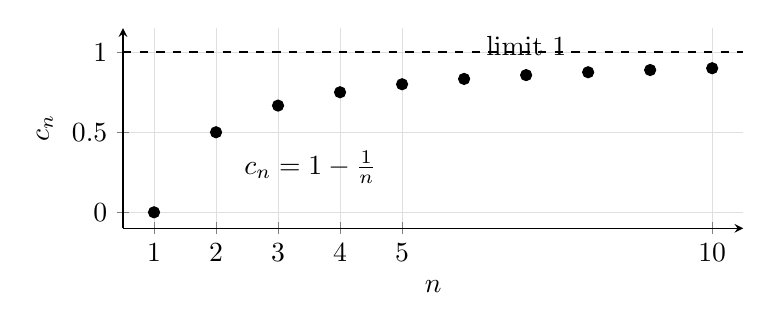
\begin{tikzpicture}
\begin{axis}[
    width=0.78\textwidth,
    height=0.34\textwidth,
    xmin=0.5, xmax=10.5,
    ymin=-0.1, ymax=1.15,
    axis lines=left,
    xlabel={\(n\)},
    ylabel={\(c_n\)},
    xtick={1,2,3,4,5,10},
    ytick={0,0.5,1},
    grid=both,
    grid style={line width=.1pt, draw=gray!25},
]
\addplot[only marks, mark=*] coordinates {
    (1,0)
    (2,0.5)
    (3,0.6667)
    (4,0.75)
    (5,0.8)
    (6,0.8333)
    (7,0.8571)
    (8,0.875)
    (9,0.8889)
    (10,0.9)
};
\addplot[thick, dashed, domain=0.5:10.5, samples=2] {1};
\node[anchor=west] at (axis cs:6.2,1.04) {limit \(1\)};
\node[anchor=west] at (axis cs:2.3,0.28) {\(c_n=1-\frac1n\)};
\end{axis}
\end{tikzpicture}
\caption{The sequence \(c_n=1-\frac1n\) approaches \(1\) from below.}
\label{fig:sequence-points-approach-one}
\end{figure}

A sequence can also be given recursively.  That means each term is built from earlier
terms.

\paragraph{Example.}
Let

\[
a_0=2,
\qquad
a_{n+1}=\frac12a_n.
\]

Then

\[
a_1=1,\qquad
a_2=\frac12,\qquad
a_3=\frac14.
\]

So the sequence is

\[
2,\ 1,\ \frac12,\ \frac14,\ \frac18,\ldots.
\]

The rule does not give \(a_n\) directly.  It gives instructions for producing the next
term from the current one.

Recursive sequences are important because many algorithms work this way.  Newton's
method, Euler's method, and many population models produce a next value from a
current value.

\subsection{Convergence and divergence}
\label{subsec:sequence-convergence-divergence}

The terms of

\[
\frac1n
\]

approach \(0\).  The terms of

\[
1-\frac1n
\]

approach \(1\).  The terms of

\[
(-1)^n
\]

do not approach a single number.

This leads to the main definition.

\begin{quote}
\textbf{Convergent sequence.}
A sequence \(\{a_n\}\) \emph{converges} to \(L\) if the terms \(a_n\) get arbitrarily
close to \(L\) as \(n\) becomes large.

We write

\[
\lim_{n\to\infty}a_n=L
\]

or

\[
a_n\to L.
\]

The number \(L\) is called the \emph{limit} of the sequence.
\end{quote}

If a sequence does not converge, it \emph{diverges}.

The phrase ``arbitrarily close'' has the same meaning as it did for limits of functions.
The only difference is that the input \(n\) now runs through whole numbers.

\begin{quote}
\textbf{Precise definition of sequence convergence.}
We write

\[
\lim_{n\to\infty}a_n=L
\]

if, for every \(\varepsilon>0\), there is an integer \(N\) such that

\[
|a_n-L|<\varepsilon
\]

whenever

\[
n\ge N.
\]
\end{quote}

In words:

\[
\boxed{
\text{After some point in the list, all later terms stay within \(\varepsilon\) of \(L\).}
}
\]

The integer \(N\) depends on the allowed error \(\varepsilon\).  Smaller error usually
requires a later starting point.

\paragraph{Example: proving \(\frac1n\to0\).}
Let

\[
a_n=\frac1n.
\]

We want to prove

\[
a_n\to0.
\]

The error from \(0\) is

\[
\left|\frac1n-0\right|=\frac1n.
\]

Given an allowed error \(\varepsilon>0\), we need

\[
\frac1n<\varepsilon.
\]

This is the same as

\[
n>\frac1\varepsilon.
\]

Choose an integer \(N\) such that

\[
N>\frac1\varepsilon.
\]

Then for every \(n\ge N\),

\[
\frac1n\le \frac1N<\varepsilon.
\]

Therefore

\[
\boxed{
\frac1n\to0.
}
\]

The proof contains the whole pattern: start with a desired error, then find how far out
in the sequence we must go.

\paragraph{Example: a sequence approaching \(1\).}
Let

\[
a_n=\frac{n}{n+1}.
\]

Rewrite:

\[
a_n=1-\frac1{n+1}.
\]

So the error from \(1\) is

\[
|a_n-1|
=
\left|-\frac1{n+1}\right|
=
\frac1{n+1}.
\]

As \(n\to\infty\), this error approaches \(0\).  Therefore

\[
\boxed{
\lim_{n\to\infty}\frac{n}{n+1}=1.
}
\]

\paragraph{Example: divergence by oscillation.}
The sequence

\[
a_n=(-1)^n
\]

does not converge.  Its terms are

\[
-1,\ 1,\ -1,\ 1,\ldots.
\]

They do not settle near one number.

If someone claims the limit is \(1\), then every odd term is distance \(2\) away from
\(1\).  If someone claims the limit is \(-1\), then every even term is distance \(2\) away
from \(-1\).  If someone claims any other number, the sequence still has two separate
clusters.

So

\[
\boxed{
(-1)^n \text{ diverges.}
}
\]

\paragraph{Example: divergence to infinity.}
The sequence

\[
a_n=n^2
\]

does not approach a finite number.  The terms grow without bound:

\[
1,\ 4,\ 9,\ 16,\ldots.
\]

We write

\[
a_n\to\infty
\]

to express this growth.  This is not convergence to a real number.  It is a precise way
of saying that the terms eventually exceed every fixed bound.

\begin{quote}
\textbf{Divergence to infinity.}
We write

\[
a_n\to\infty
\]

if, for every number \(M\), there is an integer \(N\) such that

\[
a_n>M
\]

whenever \(n\ge N\).
\end{quote}

The symbol \(\infty\) is not a number.  It describes unbounded growth.

\subsection{Basic limit laws for sequences}
\label{subsec:basic-limit-laws-sequences}

Sequence limits obey the same algebraic laws as function limits.

\begin{quote}
\textbf{Limit laws for sequences.}
Suppose

\[
a_n\to A
\qquad\text{and}\qquad
b_n\to B.
\]

Then

\[
a_n+b_n\to A+B,
\]

\[
a_n-b_n\to A-B,
\]

\[
ca_n\to cA
\]

for every constant \(c\), and

\[
a_nb_n\to AB.
\]

If \(B\neq0\) and \(b_n\neq0\) for all sufficiently large \(n\), then

\[
\frac{a_n}{b_n}\to \frac AB.
\]
\end{quote}

These laws let us compute many sequence limits by separating simple parts.

\paragraph{Example.}
Find

\[
\lim_{n\to\infty}\frac{3n^2+2n-5}{n^2-4}.
\]

Divide numerator and denominator by \(n^2\):

\[
\frac{3n^2+2n-5}{n^2-4}
=
\frac{3+\frac2n-\frac5{n^2}}{1-\frac4{n^2}}.
\]

Since

\[
\frac1n\to0
\qquad\text{and}\qquad
\frac1{n^2}\to0,
\]

we get

\[
\lim_{n\to\infty}\frac{3+\frac2n-\frac5{n^2}}{1-\frac4{n^2}}
=
\frac{3+0-0}{1-0}
=
\boxed{3}.
\]

\paragraph{Example.}
Find

\[
\lim_{n\to\infty}\frac{5n-1}{2n+7}.
\]

Divide by \(n\):

\[
\frac{5n-1}{2n+7}
=
\frac{5-\frac1n}{2+\frac7n}.
\]

Therefore

\[
\lim_{n\to\infty}\frac{5n-1}{2n+7}
=
\boxed{\frac52}.
\]

\paragraph{A warning about sampling.}
A sequence is a list, not a continuous curve.  Even when a formula involves a familiar
continuous function, the sampled values may not settle.

For example,

\[
a_n=\sin\left(\frac{n\pi}{2}\right)
\]

gives

\[
1,\ 0,\ -1,\ 0,\ 1,\ 0,\ -1,\ldots.
\]

So

\[
\sin\left(\frac{n\pi}{2}\right)
\]

does not have a limit as \(n\to\infty\).

\subsection{Monotone bounded sequences}
\label{subsec:monotone-bounded-sequences}

Some sequences converge because they are trapped.

Consider

\[
a_n=1-\frac1n.
\]

The terms increase:

\[
0,\ \frac12,\ \frac23,\ \frac34,\ldots.
\]

They never pass \(1\).  So they move upward but are bounded above.  The real line has
no gaps, so the sequence has somewhere to land.

That idea is important enough to name.

\begin{quote}
\textbf{Monotone sequences.}
A sequence \(\{a_n\}\) is \emph{increasing} if

\[
a_{n+1}\ge a_n
\]

for every \(n\).

It is \emph{decreasing} if

\[
a_{n+1}\le a_n
\]

for every \(n\).

A sequence is \emph{monotone} if it is increasing or decreasing.
\end{quote}

We also need boundedness.

\begin{quote}
\textbf{Bounded sequences.}
A sequence \(\{a_n\}\) is \emph{bounded above} if there is a number \(M\) such that

\[
a_n\le M
\]

for every \(n\).

It is \emph{bounded below} if there is a number \(m\) such that

\[
m\le a_n
\]

for every \(n\).

It is \emph{bounded} if it is bounded above and bounded below.
\end{quote}

\paragraph{Example.}
The sequence

\[
a_n=1-\frac1n
\]

is increasing and bounded above by \(1\).  It converges to \(1\).

The sequence

\[
b_n=\frac1n
\]

is decreasing and bounded below by \(0\).  It converges to \(0\).

\begin{quote}
\textbf{Monotone Convergence Theorem.}
Every increasing sequence that is bounded above converges.

Every decreasing sequence that is bounded below converges.
\end{quote}

This theorem depends on the completeness of the real numbers: the real line has no
holes.  Chapter \ref{chap:numbers-functions-models} introduced this idea through least
upper bounds and nested intervals.

\paragraph{Idea of the proof.}
Suppose \(\{a_n\}\) is increasing and bounded above.  The set of all terms

\[
\{a_1,a_2,a_3,\ldots\}
\]

has a least upper bound.  Call it \(L\).

Because \(L\) is the least upper bound, the terms must get arbitrarily close to \(L\) from
below.  If they did not, then for some \(\varepsilon>0\) all terms would satisfy

\[
a_n\le L-\varepsilon.
\]

But then \(L-\varepsilon\) would be an upper bound smaller than \(L\), contradicting
that \(L\) was the least upper bound.

So for every \(\varepsilon>0\), at least one term enters the interval

\[
(L-\varepsilon,L].
\]

Since the sequence is increasing, all later terms stay in that interval.  Therefore

\[
a_n\to L.
\]

The decreasing case is similar, using a greatest lower bound.

\paragraph{Why both hypotheses matter.}
We need monotonicity and boundedness.

The sequence

\[
a_n=n
\]

is increasing, but it is not bounded above.  It diverges to infinity.

The sequence

\[
b_n=(-1)^n
\]

is bounded, because

\[
-1\le b_n\le1
\]

for every \(n\).  But it is not monotone, and it does not converge.

\[
\boxed{
\text{Monotone alone is not enough.  Bounded alone is not enough.}
}
\]

\paragraph{Example: a sequence of finite accumulated sums.}
Define

\[
a_n=1+\frac12+\frac14+\cdots+\frac1{2^{n-1}},
\qquad n\ge1.
\]

The first few terms are

\[
a_1=1,
\qquad
a_2=\frac32,
\qquad
a_3=\frac74,
\qquad
a_4=\frac{15}{8}.
\]

The sequence is increasing because each new term adds a positive number.

It is also bounded above by \(2\).  To see this, use the finite geometric sum formula:

\[
a_n
=
\frac{1-\left(\frac12\right)^n}{1-\frac12}
=
2\left(1-\frac1{2^n}\right)
=
2-\frac1{2^{n-1}}.
\]

So

\[
a_n<2
\]

for every \(n\).  Therefore the sequence converges.  In fact,

\[
a_n\to2.
\]

This example is the first shadow of an infinite series.  The sequence \(a_n\) is made by
adding more and more terms.

\subsection{Recursive sequences and fixed points}
\label{subsec:recursive-sequences-fixed-points}

A recursive sequence gives a starting value and a rule for the next value:

\[
a_0 \quad\text{is given},
\qquad
a_{n+1}=F(a_n).
\]

If the sequence converges, say

\[
a_n\to L,
\]

then the next terms should converge to the same limit:

\[
a_{n+1}\to L.
\]

If \(F\) is continuous, we may pass to the limit in

\[
a_{n+1}=F(a_n)
\]

and get

\[
L=F(L).
\]

A number satisfying

\[
F(L)=L
\]

is called a fixed point of \(F\).

\begin{quote}
\textbf{Fixed point.}
A number \(L\) is a \emph{fixed point} of a function \(F\) if

\[
F(L)=L.
\]

If a recursive sequence

\[
a_{n+1}=F(a_n)
\]

converges to \(L\), and \(F\) is continuous at \(L\), then \(L\) must be a fixed point of
\(F\).
\end{quote}

The words ``if it converges'' are essential.  The fixed-point equation can identify a
possible limit.  It does not by itself prove that the sequence converges.

\paragraph{Example: halfway to a target.}
Let

\[
a_0=0,
\qquad
a_{n+1}=\frac{a_n+3}{2}.
\]

Each step moves halfway from the current value to \(3\).

The first few terms are

\[
0,\quad
\frac32,\quad
\frac94,\quad
\frac{21}{8},\quad
\frac{45}{16},\ldots.
\]

The terms appear to approach \(3\).

First show that they stay below \(3\).  If \(a_n<3\), then

\[
a_{n+1}=\frac{a_n+3}{2}<\frac{3+3}{2}=3.
\]

Since \(a_0=0<3\), induction gives

\[
a_n<3
\]

for every \(n\).

Now show that the sequence increases.  Compute

\[
a_{n+1}-a_n
=
\frac{a_n+3}{2}-a_n
=
\frac{3-a_n}{2}.
\]

Since \(a_n<3\), this difference is positive.  Therefore

\[
a_{n+1}>a_n.
\]

The sequence is increasing and bounded above by \(3\).  By the Monotone Convergence
Theorem, it converges.

Let its limit be \(L\).  Passing to the limit in the recursion gives

\[
L=\frac{L+3}{2}.
\]

Thus

\[
2L=L+3,
\]

so

\[
\boxed{L=3.}
\]

The sequence converges to \(3\).

\begin{figure}[h]
\centering
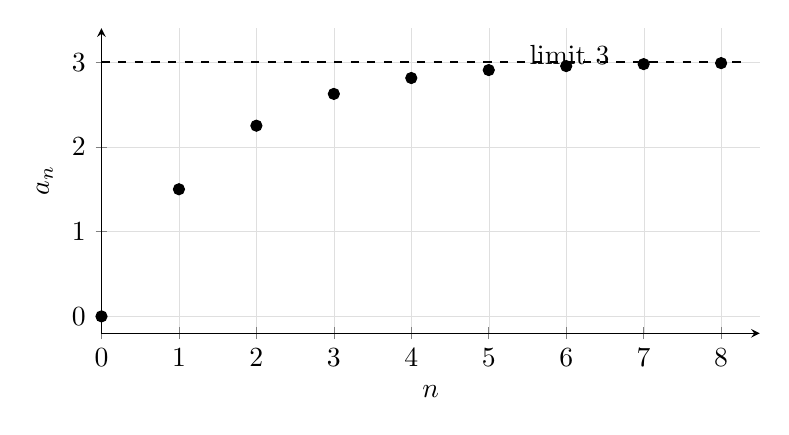
\begin{tikzpicture}
\begin{axis}[
    width=0.82\textwidth,
    height=0.45\textwidth,
    xmin=0, xmax=8.5,
    ymin=-0.2, ymax=3.4,
    axis lines=left,
    xlabel={\(n\)},
    ylabel={\(a_n\)},
    xtick={0,1,2,3,4,5,6,7,8},
    ytick={0,1,2,3},
    grid=both,
    grid style={line width=.1pt, draw=gray!25},
]
\addplot[only marks, mark=*] coordinates {
    (0,0)
    (1,1.5)
    (2,2.25)
    (3,2.625)
    (4,2.8125)
    (5,2.90625)
    (6,2.953125)
    (7,2.9765625)
    (8,2.98828125)
};
\addplot[thick, dashed, domain=0:8.3, samples=2] {3};
\node[anchor=west] at (axis cs:5.4,3.08) {limit \(3\)};
\end{axis}
\end{tikzpicture}
\caption{The recursion \(a_{n+1}=(a_n+3)/2\) moves halfway to \(3\) at each step.}
\label{fig:recursive-halfway-to-three}
\end{figure}

\paragraph{Example: fixed point is not enough.}
Consider

\[
a_0=0,
\qquad
a_{n+1}=2-a_n.
\]

The function

\[
F(x)=2-x
\]

has a fixed point, because

\[
L=2-L
\]

gives

\[
L=1.
\]

But the sequence itself is

\[
0,\ 2,\ 0,\ 2,\ 0,\ 2,\ldots.
\]

It does not converge to \(1\).  It does not converge at all.

The fixed-point equation found a possible landing place, but the sequence never lands.

\begin{quote}
\textbf{Moral.}
For a recursive sequence, the equation

\[
L=F(L)
\]

can identify possible limits.  It does not prove convergence.  To prove convergence, we
need more information, such as monotonicity and boundedness, or another argument that
controls the iteration.
\end{quote}

The next section uses sequences in a new way.  Instead of studying a list of terms
directly, we build a new sequence by adding the first \(n\) terms.  If those partial sums
settle toward a limit, we will call the result an infinite sum.

\section{Infinite series}
\label{sec:infinite-series}

A sequence is an infinite list.

A series is an infinite sum.

But an infinite sum cannot mean that we literally finish adding infinitely many numbers.
There is no last step.  The only honest definition is through limits.

We add finitely many terms, watch the partial sums, and ask whether those partial sums
approach a number.

\[
\boxed{
\text{An infinite series is a limit of finite sums.}
}
\]

\subsection{Partial sums}
\label{subsec:partial-sums}

Suppose we start with a sequence

\[
a_1,\ a_2,\ a_3,\ldots.
\]

The associated series is written

\[
\sum_{k=1}^{\infty}a_k
=
a_1+a_2+a_3+\cdots.
\]

The \(n\)-th partial sum is

\[
S_n=a_1+a_2+\cdots+a_n.
\]

In sigma notation,

\[
S_n=\sum_{k=1}^{n}a_k.
\]

So the infinite series produces a sequence of partial sums:

\[
S_1,\ S_2,\ S_3,\ldots.
\]

\begin{quote}
\textbf{Partial sums.}
Given a sequence \(\{a_k\}\), define

\[
S_n=\sum_{k=1}^{n}a_k.
\]

The sequence \(\{S_n\}\) is called the sequence of \emph{partial sums}.
\end{quote}

The infinite series converges if the partial sums converge.

\begin{quote}
\textbf{Convergence of a series.}
The series

\[
\sum_{k=1}^{\infty}a_k
\]

\emph{converges} to \(S\) if its partial sums satisfy

\[
S_n\to S.
\]

In that case, we write

\[
\sum_{k=1}^{\infty}a_k=S.
\]

If the partial sums do not converge, the series \emph{diverges}.
\end{quote}

This definition is the key.  The series is not judged by the individual terms alone.  It is
judged by the accumulated sums.

\paragraph{Example: adding halves.}
Consider

\[
\frac12+\frac14+\frac18+\frac1{16}+\cdots.
\]

The partial sums are

\[
S_1=\frac12,
\]

\[
S_2=\frac12+\frac14=\frac34,
\]

\[
S_3=\frac12+\frac14+\frac18=\frac78,
\]

and

\[
S_4=\frac{15}{16}.
\]

The pattern is

\[
S_n=1-\frac1{2^n}.
\]

Since

\[
\frac1{2^n}\to0,
\]

we get

\[
S_n\to1.
\]

Therefore

\[
\boxed{
\frac12+\frac14+\frac18+\frac1{16}+\cdots=1.
}
\]

\begin{figure}[h]
\centering
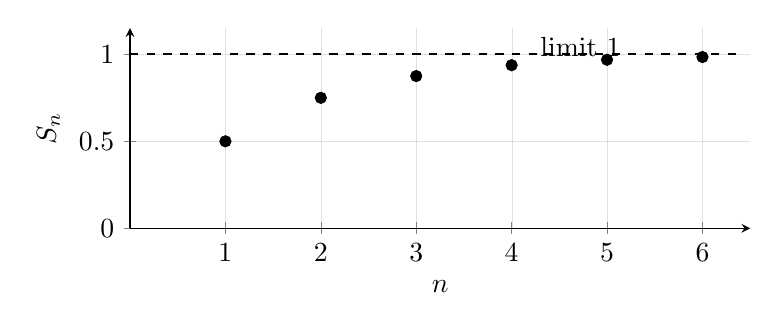
\begin{tikzpicture}
\begin{axis}[
    width=0.78\textwidth,
    height=0.34\textwidth,
    xmin=0, xmax=6.5,
    ymin=0, ymax=1.15,
    axis lines=left,
    xlabel={\(n\)},
    ylabel={\(S_n\)},
    xtick={1,2,3,4,5,6},
    ytick={0,0.5,1},
    grid=both,
    grid style={line width=.1pt, draw=gray!25},
]
\addplot[only marks, mark=*] coordinates {
    (1,0.5)
    (2,0.75)
    (3,0.875)
    (4,0.9375)
    (5,0.96875)
    (6,0.984375)
};
\addplot[thick, dashed, domain=0:6.4, samples=2] {1};
\node[anchor=west] at (axis cs:4.2,1.04) {limit \(1\)};
\end{axis}
\end{tikzpicture}
\caption{The partial sums \(S_n=\frac12+\frac14+\cdots+\frac1{2^n}\) approach \(1\).}
\label{fig:partial-sums-halves}
\end{figure}

The picture has the same structure as many earlier parts of calculus.  An infinite
process is understood through a sequence of finite approximations.

\subsection{Series convergence as a sequence problem}
\label{subsec:series-convergence-as-sequence-problem}

The definition of a series turns every convergence question into a sequence question.

\[
\sum_{k=1}^{\infty}a_k
\quad\text{converges}
\]

means

\[
S_n=a_1+a_2+\cdots+a_n
\quad\text{converges}.
\]

So when we test a series, we are really testing the behavior of its partial sums.

\paragraph{Example: a divergent series.}
Consider

\[
1+1+1+1+\cdots.
\]

The partial sums are

\[
S_1=1,
\qquad
S_2=2,
\qquad
S_3=3,
\qquad
S_n=n.
\]

Since

\[
S_n\to\infty,
\]

the series diverges.

\[
\boxed{
\sum_{k=1}^{\infty}1 \text{ diverges.}
}
\]

\paragraph{Example: partial sums can oscillate.}
Consider

\[
1-1+1-1+1-1+\cdots.
\]

The partial sums are

\[
S_1=1,
\qquad
S_2=0,
\qquad
S_3=1,
\qquad
S_4=0.
\]

So the partial sums are

\[
1,\ 0,\ 1,\ 0,\ldots.
\]

They do not approach a single number.  Therefore the series diverges.

\[
\boxed{
1-1+1-1+\cdots \text{ diverges.}
}
\]

This example is a useful warning.  Alternating signs may create cancellation, but
cancellation alone does not guarantee convergence.

\paragraph{A language point.}
It is common to say ``the series \(\sum a_k\) converges.''  Strictly speaking, the
sequence of partial sums converges.

The shorter phrase is harmless once the definition is understood.

\[
\boxed{
\text{A series converges exactly when its partial sums converge.}
}
\]

\subsection{Geometric series}
\label{subsec:geometric-series}

The most important first example of a series is the geometric series.

A geometric series has a constant ratio from one term to the next:

\[
a+ar+ar^2+ar^3+\cdots.
\]

The number \(a\) is the first term, and \(r\) is the common ratio.

\paragraph{Seed example.}
The series

\[
1+\frac12+\frac14+\frac18+\cdots
\]

is geometric with

\[
a=1,
\qquad
r=\frac12.
\]

Its partial sums, starting with \(k=0\), are

\[
S_n=1+\frac12+\frac14+\cdots+\frac1{2^n}.
\]

The formula is

\[
S_n=2-\frac1{2^n}.
\]

Therefore

\[
S_n\to2.
\]

So

\[
\boxed{
1+\frac12+\frac14+\frac18+\cdots=2.
}
\]

The same idea works for every geometric series.

\begin{quote}
\textbf{Finite geometric sum.}
If \(r\neq1\), then

\[
\boxed{
a+ar+ar^2+\cdots+ar^n
=
a\,\frac{1-r^{n+1}}{1-r}.
}
\]
\end{quote}

\paragraph{Proof.}
Let

\[
S_n=a+ar+ar^2+\cdots+ar^n.
\]

Multiply by \(r\):

\[
rS_n=ar+ar^2+ar^3+\cdots+ar^{n+1}.
\]

Subtract:

\[
S_n-rS_n
=
a-ar^{n+1}.
\]

So

\[
(1-r)S_n=a(1-r^{n+1}).
\]

Since \(r\neq1\),

\[
S_n=a\,\frac{1-r^{n+1}}{1-r}.
\]

\begin{quote}
\textbf{Geometric series.}
The infinite geometric series

\[
\sum_{k=0}^{\infty}ar^k
=
a+ar+ar^2+\cdots
\]

converges if

\[
|r|<1.
\]

In that case,

\[
\boxed{
\sum_{k=0}^{\infty}ar^k=\frac{a}{1-r}.
}
\]
\end{quote}

\paragraph{Why.}
The partial sums are

\[
S_n=a\,\frac{1-r^{n+1}}{1-r}.
\]

If

\[
|r|<1,
\]

then

\[
r^{n+1}\to0.
\]

Therefore

\[
S_n\to a\,\frac{1-0}{1-r}
=
\frac{a}{1-r}.
\]

\paragraph{Why the condition \(|r|<1\) matters.}
If \(|r|<1\), the powers

\[
r^n
\]

shrink to \(0\).  The tail of the series becomes smaller and smaller.

If \(r=1\), then

\[
a+ar+ar^2+\cdots=a+a+a+\cdots,
\]

which diverges unless \(a=0\).

If \(r=-1\), then

\[
a+ar+ar^2+\cdots=a-a+a-a+\cdots,
\]

and the partial sums oscillate.

If \(|r|>1\), then the terms do not even approach \(0\).  The partial sums cannot
settle.

\[
\boxed{
\text{A nonzero geometric series converges exactly when \(|r|<1\).}
}
\]

\paragraph{Example.}
Evaluate

\[
\sum_{k=0}^{\infty}3\left(\frac14\right)^k.
\]

This is geometric with

\[
a=3,
\qquad
r=\frac14.
\]

Since

\[
\left|\frac14\right|<1,
\]

the series converges, and

\[
\sum_{k=0}^{\infty}3\left(\frac14\right)^k
=
\frac{3}{1-\frac14}
=
\frac{3}{\frac34}
=
\boxed{4}.
\]

\paragraph{A useful tail formula.}
If

\[
|r|<1,
\]

then the part of the geometric series after the \(n\)-th term is

\[
ar^{n+1}+ar^{n+2}+ar^{n+3}+\cdots.
\]

This is another geometric series, with first term \(ar^{n+1}\) and ratio \(r\).  Therefore

\[
\boxed{
\sum_{k=n+1}^{\infty} ar^k
=
\frac{ar^{n+1}}{1-r}.
}
\]

This formula is the first clean example of a \emph{remainder} or \emph{tail}.  It tells us
exactly how much is left after a finite partial sum.

For example,

\[
1+\frac12+\frac14+\cdots+\frac1{2^n}
\]

misses the full sum \(2\) by

\[
\frac{(1/2)^{n+1}}{1-\frac12}
=
\frac1{2^n}.
\]

So the approximation improves by a factor of \(2\) each time we add one more term.

\paragraph{Example: a decimal as a series.}
The decimal

\[
0.999\ldots
\]

means

\[
\frac9{10}+\frac9{100}+\frac9{1000}+\cdots.
\]

This is geometric with

\[
a=\frac9{10},
\qquad
r=\frac1{10}.
\]

Therefore

\[
0.999\ldots
=
\frac{\frac9{10}}{1-\frac1{10}}
=
\frac{\frac9{10}}{\frac9{10}}
=
\boxed{1}.
\]

This is not a trick.  The decimal is defined by the limit of its finite truncations:

\[
0.9,\quad 0.99,\quad 0.999,\quad\ldots.
\]

Those truncations form a sequence whose limit is \(1\).

\paragraph{Example: a bouncing ball.}
A ball is dropped from a height of \(10\) feet.  Each bounce rises to \(60\%\) of the
previous height.  How far does the ball travel before coming to rest?

The ball first falls

\[
10
\]

feet.

Then it rises

\[
10(0.6)
\]

feet and falls the same distance.  Then it rises

\[
10(0.6)^2
\]

feet and falls the same distance, and so on.

So the total distance is

\[
10+2\left[10(0.6)+10(0.6)^2+10(0.6)^3+\cdots\right].
\]

The bracketed series is geometric with first term

\[
10(0.6)=6
\]

and ratio

\[
0.6.
\]

Its sum is

\[
\frac{6}{1-0.6}=\frac6{0.4}=15.
\]

Therefore the total distance is

\[
10+2(15)=\boxed{40}
\]

feet.

The model contains infinitely many smaller and smaller bounces.  A geometric series
gives their total distance.

\subsection{Telescoping series}
\label{subsec:telescoping-series}

Some series converge because most terms cancel.

Consider

\[
\sum_{k=1}^{\infty}\left(\frac1k-\frac1{k+1}\right).
\]

The \(n\)-th partial sum is

\[
S_n
=
\left(1-\frac12\right)
+
\left(\frac12-\frac13\right)
+
\left(\frac13-\frac14\right)
+\cdots+
\left(\frac1n-\frac1{n+1}\right).
\]

Everything in the middle cancels:

\[
S_n=1-\frac1{n+1}.
\]

Therefore

\[
S_n\to1.
\]

So

\[
\boxed{
\sum_{k=1}^{\infty}\left(\frac1k-\frac1{k+1}\right)=1.
}
\]

This is called a telescoping series because the sum collapses like a telescope.

\begin{quote}
\textbf{Telescoping strategy.}
To evaluate a telescoping series:

\begin{enumerate}
\item Write the \(n\)-th partial sum.
\item Expand enough terms to see the cancellation.
\item Simplify \(S_n\).
\item Take the limit as \(n\to\infty\).
\end{enumerate}
\end{quote}

\paragraph{Example: partial fractions create telescoping.}
Evaluate

\[
\sum_{k=1}^{\infty}\frac1{k(k+1)}.
\]

First decompose:

\[
\frac1{k(k+1)}
=
\frac1k-\frac1{k+1}.
\]

Therefore

\[
\sum_{k=1}^{\infty}\frac1{k(k+1)}
=
\sum_{k=1}^{\infty}\left(\frac1k-\frac1{k+1}\right).
\]

From the previous calculation,

\[
\boxed{
\sum_{k=1}^{\infty}\frac1{k(k+1)}=1.
}
\]

\paragraph{Example: cancellation does not always mean convergence.}
Consider

\[
\sum_{k=1}^{\infty}\left(\sqrt{k+1}-\sqrt{k}\right).
\]

The \(n\)-th partial sum is

\[
S_n
=
(\sqrt2-\sqrt1)
+
(\sqrt3-\sqrt2)
+
(\sqrt4-\sqrt3)
+\cdots+
(\sqrt{n+1}-\sqrt n).
\]

The middle terms cancel, leaving

\[
S_n=\sqrt{n+1}-1.
\]

But

\[
\sqrt{n+1}-1\to\infty.
\]

Therefore the series diverges.

\[
\boxed{
\sum_{k=1}^{\infty}\left(\sqrt{k+1}-\sqrt{k}\right)
\text{ diverges.}
}
\]

The cancellation was real, but the leftover endpoint still grew without bound.

\begin{quote}
\textbf{Warning.}
For a telescoping series, cancellation is only the first step.  The simplified partial sums
must still have a limit.
\end{quote}

\subsection{What series add to calculus}
\label{subsec:what-series-add-to-calculus}

A finite sum is arithmetic.  An infinite series is calculus because it is a limit:

\[
\sum_{k=1}^{\infty}a_k
=
\lim_{n\to\infty}\sum_{k=1}^{n}a_k.
\]

The first examples were friendly because we could find exact formulas for the partial
sums.

\[
\text{geometric series}
\quad\Longrightarrow\quad
S_n=a\,\frac{1-r^{n+1}}{1-r},
\]

\[
\text{telescoping series}
\quad\Longrightarrow\quad
\text{massive cancellation}.
\]

Most series will not be so generous.  We will not usually have a simple formula for
\(S_n\).  Instead, we will need tests that decide whether the partial sums converge
without computing them exactly.

The first warning is close at hand.

For a series to converge, its terms must get small.  But small terms are not enough.

The next section begins with the series

\[
1+\frac12+\frac13+\frac14+\cdots.
\]

Its terms approach \(0\).  The surprise is that the sum still diverges.

% Requires in the preamble:
% \usepackage{amsmath,amssymb}
% \usepackage{tikz,pgfplots}
% \usetikzlibrary{decorations.pathreplacing}
% \pgfplotsset{compat=1.18}

\section{The harmonic series and first warnings}
\label{sec:harmonic-series-first-warnings}

The last section gave two friendly kinds of series.  A geometric series has partial sums
with a formula.  A telescoping series has partial sums with cancellation.

Most series are less generous.  We often cannot compute

\[
S_n=a_1+a_2+\cdots+a_n
\]

exactly.  We need tests that tell whether the partial sums settle down.

The first test is not a convergence test.  It is a warning test.

\[
\boxed{
\text{If an infinite sum converges, the terms being added must become small.}
}
\]

That sounds obvious.  The danger is the converse.  Terms can become small and still add
up to infinity.

\subsection{Terms can go to zero while the series diverges}
\label{subsec:terms-zero-series-diverges}

Look at the series

\[
1+\frac12+\frac13+\frac14+\frac15+\cdots.
\]

Its terms are

\[
a_k=\frac1k.
\]

These terms approach zero:

\[
\frac1k\to0.
\]

So each individual term becomes tiny.  But the accumulated sum is another question.
The first few partial sums are

\[
S_1=1,
\]

\[
S_2=1+\frac12=1.5,
\]

\[
S_3=1+\frac12+\frac13\approx1.833,
\]

\[
S_4=1+\frac12+\frac13+\frac14\approx2.083.
\]

The partial sums keep increasing.  That alone does not prove divergence.  They might
increase toward a horizontal ceiling, as the geometric partial sums did.

The surprise is that there is no ceiling.

The series

\[
\sum_{k=1}^{\infty}\frac1k
\]

is called the \emph{harmonic series}.  It diverges, even though its terms approach
zero.

This is the first essential warning in infinite series:

\[
\boxed{
 a_k\to0 \quad \text{does not imply} \quad \sum_{k=1}^{\infty}a_k \text{ converges.}
}
\]

A term is one small contribution.  A series is the accumulated effect of infinitely many
contributions.  Small pieces can still have an infinite total.

\subsection{A necessary condition for convergence}
\label{subsec:necessary-condition-for-series-convergence}

There is one statement we can prove immediately.

Suppose the series

\[
\sum_{k=1}^{\infty}a_k
\]

converges.  Its partial sums

\[
S_n=a_1+a_2+\cdots+a_n
\]

approach some number \(S\):

\[
S_n\to S.
\]

The term \(a_n\) is the difference between two consecutive partial sums:

\[
a_n=S_n-S_{n-1},
\qquad n\ge2.
\]

Since

\[
S_n\to S
\qquad\text{and}\qquad
S_{n-1}\to S,
\]

we get

\[
a_n=S_n-S_{n-1}\to S-S=0.
\]

So the terms of a convergent series must approach zero.

\begin{quote}
\textbf{Necessary condition for convergence.}
If

\[
\sum_{k=1}^{\infty}a_k
\]

converges, then

\[
\boxed{a_k\to0.}
\]

Equivalently, if \(a_k\) does not approach \(0\), then

\[
\boxed{\sum_{k=1}^{\infty}a_k \text{ diverges.}}
\]
\end{quote}

The second form is often called the \emph{term test for divergence}.

The name matters.  It is a divergence test, not a convergence test.

\[
\boxed{
\text{If the terms do not go to zero, the series diverges.}
}
\]

But if the terms do go to zero, we still do not know.

\paragraph{Example: terms do not go to zero.}
Show that

\[
\sum_{k=1}^{\infty}\frac{k}{k+1}
\]

diverges.

The terms are

\[
a_k=\frac{k}{k+1}.
\]

Since

\[
\frac{k}{k+1}=\frac{1}{1+\frac1k}\to1,
\]

the terms do not approach zero.  Therefore the series diverges.

\[
\boxed{
\sum_{k=1}^{\infty}\frac{k}{k+1} \text{ diverges.}
}
\]

There is no need to study the partial sums.  The individual terms are already too large
to allow convergence.

\paragraph{Example: oscillating terms.}
The series

\[
\sum_{k=1}^{\infty}(-1)^k
\]

has terms

\[
-1,
\quad 1,
\quad -1,
\quad 1,
\quad\ldots.
\]

The terms do not approach zero.  Therefore the series diverges.

This agrees with what we saw from partial sums:

\[
-1,
\quad 0,
\quad -1,
\quad 0,
\quad\ldots.
\]

The partial sums oscillate instead of approaching a number.

\paragraph{Example: terms go to zero, but the test says nothing.}
For the harmonic series,

\[
a_k=\frac1k\to0.
\]

The term test gives no conclusion.  It does not say the harmonic series converges.
It only says that the first obstacle to convergence has been passed.

We need another idea.

\subsection{The harmonic series}
\label{subsec:harmonic-series}

The harmonic series is

\[
\boxed{
\sum_{k=1}^{\infty}\frac1k
=1+\frac12+\frac13+\frac14+\cdots.
}
\]

It is the simplest series whose terms go to zero but whose sum still diverges.

The partial sums grow slowly:

\[
\begin{array}{c|c}
 n & S_n=1+\frac12+\cdots+\frac1n \\ \hline
 1 & 1 \\
 2 & 1.5 \\
 4 & 2.083\ldots \\
 8 & 2.718\ldots \\
 16 & 3.381\ldots
\end{array}
\]

Slow growth can look like convergence if we only compute a few terms.  This is a
common trap in numerical work.  A long plateau is not the same as a limit.

The right proof groups the terms.

\subsection{Grouping terms to see divergence}
\label{subsec:grouping-harmonic-divergence}

Write the harmonic series in blocks whose lengths double:

\[
1
+\frac12
+\left(\frac13+\frac14\right)
+\left(\frac15+\frac16+\frac17+\frac18\right)
+\cdots.
\]

Now estimate each block from below.

The block

\[
\frac13+\frac14
\]

has two terms, and each is at least \(1/4\).  Therefore

\[
\frac13+\frac14\ge \frac14+\frac14=\frac12.
\]

The next block

\[
\frac15+\frac16+\frac17+\frac18
\]

has four terms, and each is at least \(1/8\).  Therefore

\[
\frac15+\frac16+\frac17+\frac18
\ge
4\cdot\frac18
=
\frac12.
\]

The next block has eight terms, each at least \(1/16\), so it also contributes at least
\(1/2\).

In general, the block

\[
\frac1{2^{m-1}+1}+\frac1{2^{m-1}+2}+\cdots+\frac1{2^m}
\]

has \(2^{m-1}\) terms, and each term is at least \(1/2^m\).  Thus the block contributes
at least

\[
2^{m-1}\cdot\frac1{2^m}=\frac12.
\]

So after enough blocks, the harmonic series is at least

\[
1+\frac12+\frac12+\frac12+\cdots.
\]

More precisely,

\[
S_{2^m}
=
1+\frac12+\left(\frac13+\frac14\right)+\cdots+
\left(\frac1{2^{m-1}+1}+\cdots+\frac1{2^m}\right)
\ge
1+\frac{m}{2}.
\]

Since

\[
1+\frac{m}{2}\to\infty,
\]

the partial sums of the harmonic series are unbounded.  Therefore the harmonic series
diverges.

\[
\boxed{
\sum_{k=1}^{\infty}\frac1k \text{ diverges.}
}
\]

\begin{figure}[h]
\centering
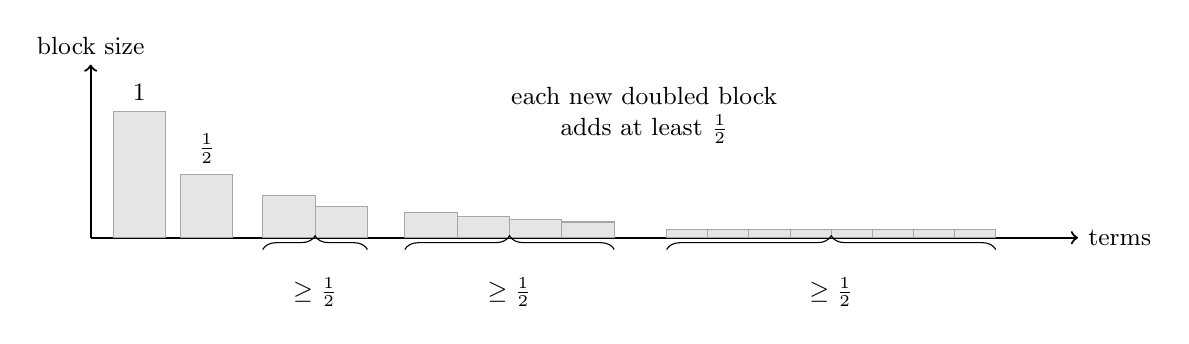
\begin{tikzpicture}[xscale=0.95, yscale=1.0, every node/.style={font=\small}]
  \draw[->, thick] (0,0) -- (13.2,0) node[right] {terms};
  \draw[->, thick] (0,0) -- (0,2.2) node[above] {block size};

  % first block
  \draw[fill=gray!20, draw=gray!70] (0.3,0) rectangle (1.0,1.6);
  \node[above] at (0.65,1.62) {\(1\)};

  % second block
  \draw[fill=gray!20, draw=gray!70] (1.2,0) rectangle (1.9,0.8);
  \node[above] at (1.55,0.82) {\(\frac12\)};

  % third block two terms
  \draw[fill=gray!20, draw=gray!70] (2.3,0) rectangle (3.0,0.533);
  \draw[fill=gray!20, draw=gray!70] (3.0,0) rectangle (3.7,0.4);
  \draw[decorate, decoration={brace, amplitude=5pt}] (2.3,-0.15) -- (3.7,-0.15);
  \node[below] at (3.0,-0.38) {\(\ge \frac12\)};

  % fourth block four terms
  \foreach \x/\h in {4.2/0.32,4.9/0.267,5.6/0.229,6.3/0.2} {
    \draw[fill=gray!20, draw=gray!70] (\x,0) rectangle +(0.7,\h);
  }
  \draw[decorate, decoration={brace, amplitude=5pt}] (4.2,-0.15) -- (7.0,-0.15);
  \node[below] at (5.6,-0.38) {\(\ge \frac12\)};

  % fifth block eight stylized terms at common lower height
  \foreach \i in {0,...,7} {
    \draw[fill=gray!20, draw=gray!70] ({7.7+0.55*\i},0) rectangle +(0.55,0.1);
  }
  \draw[decorate, decoration={brace, amplitude=5pt}] (7.7,-0.15) -- (12.1,-0.15);
  \node[below] at (9.9,-0.38) {\(\ge \frac12\)};

  \node[align=center] at (7.4,1.55) {each new doubled block\\adds at least \(\frac12\)};
\end{tikzpicture}
\caption{Grouping the harmonic series into doubled blocks shows that the partial sums keep gaining at least \(1/2\).}
\label{fig:harmonic-grouping-blocks}
\end{figure}

This proof is more than a trick.  It shows a new habit.  When we cannot compute partial
sums exactly, we compare them with something simpler.

That is the main idea behind the next tests.

\section{Positive series tests}
\label{sec:positive-series-tests}

The harmonic series was positive: every term was greater than zero.  Positive series are
easier than arbitrary series because there is no cancellation.

If

\[
a_k\ge0
\]

for every \(k\), then the partial sums

\[
S_n=a_1+a_2+\cdots+a_n
\]

are increasing:

\[
S_{n+1}=S_n+a_{n+1}\ge S_n.
\]

So a positive series has only two possibilities:

\[
\text{the partial sums are bounded above and converge,}
\]

or

\[
\text{the partial sums grow without bound and diverge.}
\]

This is the Monotone Convergence Theorem in action.

\begin{quote}
\textbf{Positive-series principle.}
For a series with nonnegative terms,

\[
\sum_{k=1}^{\infty}a_k,
\qquad a_k\ge0,
\]

the partial sums are increasing.  Therefore the series converges exactly when its partial
sums are bounded above.
\end{quote}

The tests in this section are different ways to prove boundedness or unboundedness
without knowing an exact formula for \(S_n\).

\subsection{Integral test}
\label{subsec:integral-test}

A positive decreasing sequence can be compared with the area under a positive
decreasing curve.

The harmonic series already hints at this.  The terms

\[
\frac1k
\]

come from the function

\[
f(x)=\frac1x.
\]

The improper integral

\[
\int_1^{\infty}\frac1x\,dx
\]

diverges.  The harmonic series also diverges.  This agreement is not an accident.

\begin{figure}[h]
\centering
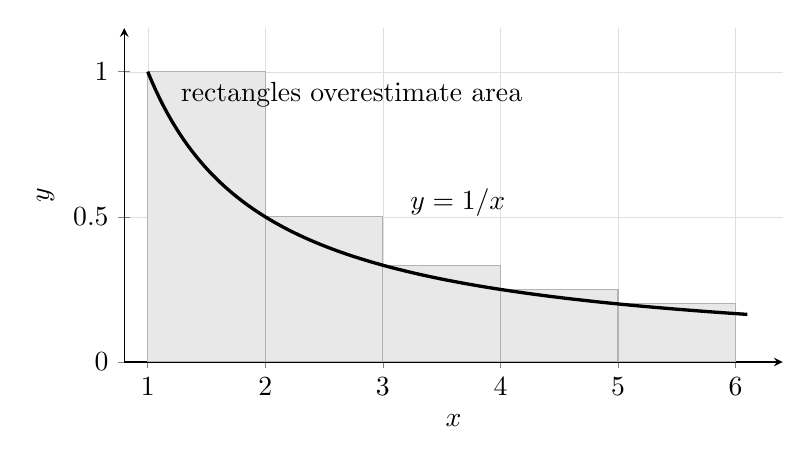
\begin{tikzpicture}
\begin{axis}[
    width=0.82\textwidth,
    height=0.48\textwidth,
    xmin=0.8, xmax=6.4,
    ymin=0, ymax=1.15,
    axis lines=left,
    xlabel={\(x\)},
    ylabel={\(y\)},
    xtick={1,2,3,4,5,6},
    ytick={0,0.5,1},
    grid=both,
    grid style={line width=.1pt, draw=gray!25},
]
% upper rectangles for f(x)=1/x, k=1..5
\draw[fill=gray!18, draw=gray!60] (axis cs:1,0) rectangle (axis cs:2,1);
\draw[fill=gray!18, draw=gray!60] (axis cs:2,0) rectangle (axis cs:3,0.5);
\draw[fill=gray!18, draw=gray!60] (axis cs:3,0) rectangle (axis cs:4,0.3333);
\draw[fill=gray!18, draw=gray!60] (axis cs:4,0) rectangle (axis cs:5,0.25);
\draw[fill=gray!18, draw=gray!60] (axis cs:5,0) rectangle (axis cs:6,0.2);
\addplot[very thick, domain=1:6.1, samples=150] {1/x};
\node[anchor=west] at (axis cs:3.15,0.55) {\(y=1/x\)};
\node[anchor=west] at (axis cs:1.2,0.92) {rectangles overestimate area};
\end{axis}
\end{tikzpicture}
\caption{For a positive decreasing function, rectangle sums and improper integrals control each other.}
\label{fig:integral-test-rectangles}
\end{figure}

The geometric comparison is simple.  Suppose \(f\) is positive and decreasing.  On the
interval \([k,k+1]\), we have

\[
f(k+1)\le f(x)\le f(k).
\]

Integrating across that interval gives

\[
f(k+1)\le \int_k^{k+1} f(x)\,dx\le f(k),
\]

because the interval has width \(1\).

Adding these inequalities connects the series to the improper integral.

\begin{quote}
\textbf{Integral Test.}
Let \(f\) be continuous, positive, and decreasing on \([1,\infty)\).  Suppose

\[
a_k=f(k).
\]

Then the series

\[
\sum_{k=1}^{\infty}a_k
\]

and the improper integral

\[
\int_1^{\infty} f(x)\,dx
\]

either both converge or both diverge.
\end{quote}

\paragraph{Why the test works.}
Let

\[
S_n=f(1)+f(2)+\cdots+f(n).
\]

Since \(f\) is decreasing,

\[
\int_1^{n+1} f(x)\,dx\le S_n.
\]

Also,

\[
S_n\le f(1)+\int_1^n f(x)\,dx.
\]

If the improper integral diverges, then the lower bound

\[
\int_1^{n+1} f(x)\,dx\le S_n
\]

forces \(S_n\to\infty\).  So the series diverges.

If the improper integral converges, then

\[
S_n\le f(1)+\int_1^{\infty}f(x)\,dx.
\]

The partial sums are increasing and bounded above.  Therefore they converge.

\paragraph{Example: a convergent positive series.}
Determine whether

\[
\sum_{k=1}^{\infty}\frac1{k^2}
\]

converges.

Use

\[
f(x)=\frac1{x^2}.
\]

This function is continuous, positive, and decreasing on \([1,\infty)\).  The improper
integral is

\[
\int_1^{\infty}\frac1{x^2}\,dx
=
\lim_{b\to\infty}\int_1^b x^{-2}\,dx.
\]

Compute:

\[
\int_1^b x^{-2}\,dx
=
\left[-\frac1x\right]_1^b
=
1-\frac1b.
\]

Let \(b\to\infty\):

\[
\int_1^{\infty}\frac1{x^2}\,dx=1.
\]

The integral converges.  Therefore

\[
\boxed{
\sum_{k=1}^{\infty}\frac1{k^2} \text{ converges.}
}
\]

The integral test tells convergence.  It does not say that the sum equals \(1\).  In fact,
the sum is larger than \(1\), because the first term alone is \(1\).

\paragraph{Example: the harmonic series again.}
Use the integral test on

\[
\sum_{k=1}^{\infty}\frac1k.
\]

Let

\[
f(x)=\frac1x.
\]

Then

\[
\int_1^{\infty}\frac1x\,dx
=
\lim_{b\to\infty}\ln b
=
\infty.
\]

The integral diverges.  Therefore

\[
\boxed{
\sum_{k=1}^{\infty}\frac1k \text{ diverges.}
}
\]

This is a second proof of the divergence of the harmonic series.  The grouping proof
showed the divergence by blocks.  The integral test shows that the same divergence is
connected to the infinite area under \(1/x\).

\paragraph{Why the hypotheses matter.}
The integral test is not a rule for every function.  It requires \(f\) to be continuous,
positive, and decreasing.

The positivity matters because the proof uses increasing partial sums and area
comparison.  If signs change, cancellation can change the behavior.

The decreasing condition matters because the rectangles must consistently sit above or
below the curve.  If the function jumps up and down, the rectangle comparison can fail.

\[
\boxed{
\text{Do not use the integral test until positivity and decreasing behavior have been checked.}
}
\]

\subsection{Remainder estimates from the integral test}
\label{subsec:integral-test-remainder-estimates}

The integral test can do more than decide convergence.  For a convergent positive
series, it can estimate the error after stopping at a finite partial sum.

Suppose

\[
\sum_{k=1}^{\infty}a_k
\]

converges, with

\[
a_k=f(k),
\]

where \(f\) is continuous, positive, and decreasing.  Let

\[
S=\sum_{k=1}^{\infty}a_k
\]

and

\[
S_n=\sum_{k=1}^{n}a_k.
\]

The remainder after \(n\) terms is

\[
R_n=S-S_n=\sum_{k=n+1}^{\infty}a_k.
\]

The same rectangle picture gives

\[
\boxed{
\int_{n+1}^{\infty}f(x)\,dx
\le
R_n
\le
\int_n^{\infty}f(x)\,dx.
}
\]

Equivalently,

\[
\boxed{
S_n+\int_{n+1}^{\infty}f(x)\,dx
\le
S
\le
S_n+\int_n^{\infty}f(x)\,dx.
}
\]

This is the kind of estimate calculus values: not only an approximation, but a bound on
how far the approximation can be from the truth.

\paragraph{Example: estimating \(\sum 1/k^2\).}
Let

\[
S=\sum_{k=1}^{\infty}\frac1{k^2}.
\]

Approximate \(S\) by the first ten terms:

\[
S_{10}=1+\frac1{2^2}+\frac1{3^2}+\cdots+\frac1{10^2}\approx1.54977.
\]

For

\[
f(x)=\frac1{x^2},
\]

the remainder satisfies

\[
\int_{11}^{\infty}\frac1{x^2}\,dx
\le
R_{10}
\le
\int_{10}^{\infty}\frac1{x^2}\,dx.
\]

Compute the two bounds:

\[
\int_{11}^{\infty}\frac1{x^2}\,dx=\frac1{11},
\qquad
\int_{10}^{\infty}\frac1{x^2}\,dx=\frac1{10}.
\]

Thus

\[
\frac1{11}\le R_{10}\le \frac1{10}.
\]

So

\[
1.54977+\frac1{11}
\le
S
\le
1.54977+\frac1{10}.
\]

Therefore

\[
\boxed{
1.64067\lesssim S\lesssim1.64977.
}
\]

The first ten terms alone do not give many correct decimal places, but the estimate is
honest.  It tells us exactly how uncertain we are.

\paragraph{How many terms are enough?}
How many terms of

\[
\sum_{k=1}^{\infty}\frac1{k^2}
\]

are needed to make the remainder less than \(0.001\)?

The upper remainder estimate is

\[
R_n\le \int_n^{\infty}\frac1{x^2}\,dx=\frac1n.
\]

We want

\[
\frac1n<0.001.
\]

So we need

\[
n>1000.
\]

Taking \(1001\) terms is enough.

This is not the most efficient way to approximate the sum, but it is reliable.  Later,
series with faster convergence will give much better approximations with far fewer terms.

\subsection{Direct comparison}
\label{subsec:direct-comparison-test}

The harmonic series and the series \(\sum 1/k^2\) now become measuring sticks.

If a positive series is smaller than a known convergent positive series, it must converge.
If it is larger than a known divergent positive series, it must diverge.

\begin{quote}
\textbf{Direct Comparison Test.}
Suppose

\[
0\le a_k\le b_k
\]

for all sufficiently large \(k\).

If

\[
\sum_{k=1}^{\infty}b_k
\]

converges, then

\[
\sum_{k=1}^{\infty}a_k
\]

also converges.

If

\[
0\le b_k\le a_k
\]

for all sufficiently large \(k\), and

\[
\sum_{k=1}^{\infty}b_k
\]

diverges, then

\[
\sum_{k=1}^{\infty}a_k
\]

also diverges.
\end{quote}

The phrase ``for all sufficiently large \(k\)'' means that finitely many early terms do not
matter.  Changing, adding, or deleting finitely many terms can change the value of a
convergent series, but it cannot change whether the series converges.

\paragraph{Why the test works.}
For positive series, partial sums increase.  If every term of \(a_k\) is eventually no
larger than the corresponding term of \(b_k\), then the partial sums of \(a_k\) are
eventually controlled by the partial sums of \(b_k\), plus a finite starting amount.

A finite starting amount cannot cause divergence.  The infinite tail decides.

\paragraph{Example: comparison with \(1/k^2\).}
Determine whether

\[
\sum_{k=1}^{\infty}\frac1{k^2+5}
\]

converges.

For every \(k\ge1\),

\[
k^2+5\ge k^2.
\]

Therefore

\[
0\le \frac1{k^2+5}\le \frac1{k^2}.
\]

We already know that

\[
\sum_{k=1}^{\infty}\frac1{k^2}
\]

converges.  By direct comparison,

\[
\boxed{
\sum_{k=1}^{\infty}\frac1{k^2+5} \text{ converges.}
}
\]

\paragraph{Example: comparison with the harmonic series.}
Determine whether

\[
\sum_{k=1}^{\infty}\frac1{\sqrt{k}}
\]

converges.

For \(k\ge1\),

\[
\sqrt{k}\le k.
\]

Taking reciprocals reverses the inequality because all quantities are positive:

\[
\frac1{\sqrt{k}}\ge \frac1k.
\]

The harmonic series

\[
\sum_{k=1}^{\infty}\frac1k
\]

diverges.  Since

\[
\frac1{\sqrt{k}}
\]

is even larger term by term, the series

\[
\boxed{
\sum_{k=1}^{\infty}\frac1{\sqrt{k}} \text{ diverges.}
}
\]

\paragraph{Example: bounding a messy numerator.}
Determine whether

\[
\sum_{k=1}^{\infty}\frac{3+\sin k}{k^2}
\]

converges.

Since

\[
-1\le \sin k\le1,
\]

we have

\[
2\le 3+\sin k\le4.
\]

Therefore

\[
0\le \frac{3+\sin k}{k^2}\le \frac4{k^2}.
\]

The series

\[
\sum_{k=1}^{\infty}\frac4{k^2}=4\sum_{k=1}^{\infty}\frac1{k^2}
\]

converges.  By direct comparison,

\[
\boxed{
\sum_{k=1}^{\infty}\frac{3+\sin k}{k^2} \text{ converges.}
}
\]

The oscillation in \(\sin k\) is harmless here because the whole term is trapped below a
convergent positive series.

\subsection{Limit comparison}
\label{subsec:limit-comparison-test}

Direct comparison requires an inequality.  Sometimes the right comparison is visible,
but the inequality is awkward.

For large \(k\), the expression

\[
\frac{3k+1}{k^2+5k}
\]

behaves like

\[
\frac{3k}{k^2}=\frac3k.
\]

So we expect the series to behave like the harmonic series and diverge.

Limit comparison turns this kind of leading-term reasoning into a test.

\begin{quote}
\textbf{Limit Comparison Test.}
Suppose

\[
a_k>0,
\qquad
b_k>0
\]

for all sufficiently large \(k\).  If

\[
\lim_{k\to\infty}\frac{a_k}{b_k}=c
\]

where

\[
0<c<\infty,
\]

then

\[
\sum_{k=1}^{\infty}a_k
\]

and

\[
\sum_{k=1}^{\infty}b_k
\]

either both converge or both diverge.
\end{quote}

\paragraph{Why the test works.}
If

\[
\frac{a_k}{b_k}\to c
\]

with \(0<c<\infty\), then for all large \(k\), the ratio \(a_k/b_k\) is trapped between two
positive constants.  For example, eventually

\[
\frac c2\le \frac{a_k}{b_k}\le 2c.
\]

So eventually

\[
\frac c2 b_k\le a_k\le 2c b_k.
\]

The two series are comparable in both directions.  Direct comparison then forces them
to have the same convergence behavior.

\paragraph{Example: behaves like \(1/k\).}
Determine whether

\[
\sum_{k=1}^{\infty}\frac{3k+1}{k^2+5k}
\]

converges.

Compare with

\[
b_k=\frac1k.
\]

Let

\[
a_k=\frac{3k+1}{k^2+5k}.
\]

Then

\[
\frac{a_k}{b_k}
=
\frac{\frac{3k+1}{k^2+5k}}{\frac1k}
=
\frac{k(3k+1)}{k^2+5k}
=
\frac{3k+1}{k+5}.
\]

Therefore

\[
\lim_{k\to\infty}\frac{a_k}{b_k}=3.
\]

Since

\[
0<3<\infty,
\]

the given series has the same convergence behavior as

\[
\sum_{k=1}^{\infty}\frac1k.
\]

The harmonic series diverges.  Therefore

\[
\boxed{
\sum_{k=1}^{\infty}\frac{3k+1}{k^2+5k} \text{ diverges.}
}
\]

\paragraph{Example: behaves like \(1/k^2\).}
Determine whether

\[
\sum_{k=1}^{\infty}\frac{5k^2+1}{k^4+k}
\]

converges.

For large \(k\), the term behaves like

\[
\frac{5k^2}{k^4}=\frac5{k^2}.
\]

Compare with

\[
b_k=\frac1{k^2}.
\]

Then

\[
\frac{a_k}{b_k}
=
\frac{\frac{5k^2+1}{k^4+k}}{\frac1{k^2}}
=
\frac{k^2(5k^2+1)}{k^4+k}
=
\frac{5k^4+k^2}{k^4+k}.
\]

Divide numerator and denominator by \(k^4\):

\[
\frac{5+\frac1{k^2}}{1+\frac1{k^3}}\to5.
\]

Since

\[
\sum_{k=1}^{\infty}\frac1{k^2}
\]

converges, the given series also converges:

\[
\boxed{
\sum_{k=1}^{\infty}\frac{5k^2+1}{k^4+k} \text{ converges.}
}
\]

\paragraph{Choosing the comparison series.}
For rational expressions in \(k\), the comparison usually comes from the highest powers.

\[
\frac{\text{polynomial of degree }m}{\text{polynomial of degree }n}
\]

behaves like

\[
\frac{\text{leading term}}{\text{leading term}}
\]

for large \(k\).  That usually points to a series of the form

\[
\sum \frac1{k^p}.
\]

These are called \(p\)-series.

\subsection{\(p\)-series}
\label{subsec:p-series}

A \emph{\(p\)-series} has the form

\[
\sum_{k=1}^{\infty}\frac1{k^p}.
\]

The harmonic series is the case \(p=1\):

\[
\sum_{k=1}^{\infty}\frac1k.
\]

The series

\[
\sum_{k=1}^{\infty}\frac1{k^2}
\]

is the case \(p=2\).

The integral test gives the full rule.

\begin{quote}
\textbf{\(p\)-series test.}
The series

\[
\sum_{k=1}^{\infty}\frac1{k^p}
\]

converges if

\[
p>1,
\]

and diverges if

\[
p\le1.
\]
\end{quote}

\paragraph{Proof for \(p>0\).}
Use

\[
f(x)=\frac1{x^p}.
\]

This function is continuous, positive, and decreasing on \([1,\infty)\) when \(p>0\).

For \(p\neq1\),

\[
\int_1^b x^{-p}\,dx
=
\left[\frac{x^{1-p}}{1-p}\right]_1^b
=
\frac{b^{1-p}-1}{1-p}.
\]

If \(p>1\), then \(1-p<0\), so

\[
b^{1-p}\to0.
\]

Thus

\[
\int_1^{\infty}\frac1{x^p}\,dx
=
\frac1{p-1},
\]

which is finite.  Therefore the \(p\)-series converges.

If \(0<p<1\), then \(1-p>0\), so

\[
b^{1-p}\to\infty.
\]

The improper integral diverges, and therefore the \(p\)-series diverges.

If \(p=1\), then

\[
\int_1^b \frac1x\,dx=\ln b\to\infty,
\]

so the harmonic series diverges.

If \(p\le0\), then the terms

\[
\frac1{k^p}=k^{-p}
\]

do not approach zero.  The series diverges by the term test.

\paragraph{Examples.}
The series

\[
\sum_{k=1}^{\infty}\frac1{k^{3/2}}
\]

converges because

\[
\frac32>1.
\]

The series

\[
\sum_{k=1}^{\infty}\frac1{\sqrt{k}}
=
\sum_{k=1}^{\infty}\frac1{k^{1/2}}
\]

diverges because

\[
\frac12\le1.
\]

The series

\[
\sum_{k=1}^{\infty}\frac1{k^{1.01}}
\]

converges, but very slowly.  The exponent is greater than \(1\), but only barely.

The series

\[
\sum_{k=1}^{\infty}\frac1{k^{0.99}}
\]

diverges, but very slowly.  The exponent is less than \(1\), but only barely.

The line \(p=1\) is the boundary.

\begin{quote}
\textbf{What to remember.}
For positive series, comparison is the central habit.

\[
\begin{array}{c|c}
\textbf{series} & \textbf{behavior} \\ \hline
\displaystyle \sum \frac1k & \text{diverges} \\[6pt]
\displaystyle \sum \frac1{k^p},\ p>1 & \text{converges} \\[6pt]
\displaystyle \sum ar^k,\ |r|<1 & \text{converges}
\end{array}
\]

When an unfamiliar positive series appears, compare it with one of these measuring
sticks.
\end{quote}

Positive series are now under partial control.  But many important series alternate signs:

\[
1-\frac12+\frac13-\frac14+\frac15-\cdots.
\]

The positive version diverges.  The alternating version behaves differently because
cancellation becomes organized.  That is the next story.

\section{Alternating series}
\label{sec:alternating-series}

Positive series have no cancellation.  Every term pushes the partial sums upward.  That
is why comparison and the integral test work so cleanly.

But many important series change sign:

\[
1-\frac12+\frac13-\frac14+\frac15-\cdots.
\]

The positive version,

\[
1+\frac12+\frac13+\frac14+\cdots,
\]

diverges.  The alternating version behaves differently because each term partially
corrects the last one.

This is the next idea:

\[
\boxed{
\text{organized cancellation can make an infinite sum converge.}
}
\]

\subsection{A first alternating sum}
\label{subsec:first-alternating-sum}

Consider

\[
1-\frac12+\frac13-\frac14+\frac15-\frac16+\cdots.
\]

The terms alternate sign.  The partial sums are

\[
S_1=1,
\]

\[
S_2=1-\frac12=\frac12,
\]

\[
S_3=1-\frac12+\frac13=\frac56,
\]

\[
S_4=1-\frac12+\frac13-\frac14=\frac7{12}.
\]

The odd partial sums are

\[
S_1,\ S_3,\ S_5,\ldots,
\]

and the even partial sums are

\[
S_2,\ S_4,\ S_6,\ldots.
\]

The odd sums come from stopping immediately after adding a positive term.  They sit
above the final value.  The even sums come from stopping immediately after subtracting
a term.  They sit below the final value.

The positive and negative corrections get smaller:

\[
1,\quad \frac12,\quad \frac13,\quad \frac14,\quad\ldots.
\]

So the partial sums bounce back and forth across a narrowing gap.

\begin{figure}[h]
\centering
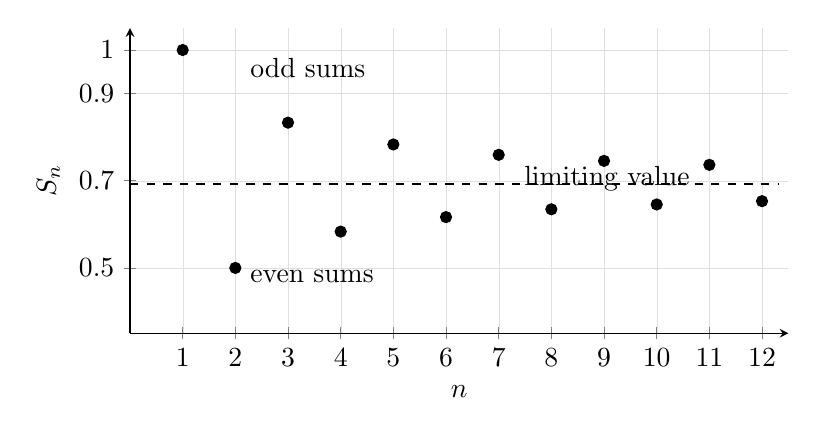
\begin{tikzpicture}
\begin{axis}[
    width=0.82\textwidth,
    height=0.45\textwidth,
    xmin=0, xmax=12.5,
    ymin=0.35, ymax=1.05,
    axis lines=left,
    xlabel={\(n\)},
    ylabel={\(S_n\)},
    xtick={1,2,3,4,5,6,7,8,9,10,11,12},
    ytick={0.5,0.7,0.9,1.0},
    grid=both,
    grid style={line width=.1pt, draw=gray!25},
]
\addplot[only marks, mark=*] coordinates {
    (1,1)
    (2,0.5)
    (3,0.833333)
    (4,0.583333)
    (5,0.783333)
    (6,0.616667)
    (7,0.759524)
    (8,0.634524)
    (9,0.745635)
    (10,0.645635)
    (11,0.736544)
    (12,0.653211)
};
\addplot[thick, dashed, domain=0:12.3, samples=2] {0.693147};
\node[anchor=west] at (axis cs:7.3,0.705) {limiting value};
\node[anchor=west] at (axis cs:2.1,0.96) {odd sums};
\node[anchor=west] at (axis cs:2.1,0.48) {even sums};
\end{axis}
\end{tikzpicture}
\caption{The alternating harmonic partial sums bounce above and below their limiting value.}
\label{fig:alternating-harmonic-partial-sums}
\end{figure}

This picture suggests convergence, but it also suggests more: the error after stopping is
controlled by the next term.

\subsection{Alternating Series Test}
\label{subsec:alternating-series-test}

An alternating series has the form

\[
\sum_{k=1}^{\infty}(-1)^{k-1}b_k
=
b_1-b_2+b_3-b_4+\cdots,
\]

or the form

\[
\sum_{k=1}^{\infty}(-1)^k b_k
=
-b_1+b_2-b_3+b_4-\cdots,
\]

where

\[
b_k\ge0.
\]

The signs alternate.  The numbers \(b_k\) are the sizes of the terms.

The clean convergence theorem requires two conditions:

\[
b_{k+1}\le b_k
\]

and

\[
b_k\to0.
\]

So the term sizes must decrease to zero.

\begin{quote}
\textbf{Alternating Series Test.}
Suppose

\[
b_k\ge0,
\qquad
b_{k+1}\le b_k,
\]

and

\[
b_k\to0.
\]

Then the alternating series

\[
\boxed{
\sum_{k=1}^{\infty}(-1)^{k-1}b_k
}
\]

converges.
\end{quote}

The same conclusion holds for

\[
\sum_{k=1}^{\infty}(-1)^k b_k,
\]

which only changes the overall sign.

\paragraph{Why the test works.}
Let

\[
S_n=b_1-b_2+b_3-b_4+\cdots+(-1)^{n-1}b_n.
\]

Look first at the even partial sums:

\[
S_2=b_1-b_2,
\]

\[
S_4=b_1-b_2+b_3-b_4,
\]

\[
S_6=b_1-b_2+b_3-b_4+b_5-b_6.
\]

Because

\[
b_3\ge b_4,
\qquad
b_5\ge b_6,
\]

each new pair adds a nonnegative amount.  Thus

\[
S_2\le S_4\le S_6\le\cdots.
\]

So the even partial sums increase.

Now look at the odd partial sums:

\[
S_1=b_1,
\]

\[
S_3=b_1-b_2+b_3,
\]

\[
S_5=b_1-b_2+b_3-b_4+b_5.
\]

Going from \(S_1\) to \(S_3\) changes the sum by

\[
-b_2+b_3\le0,
\]

because \(b_2\ge b_3\).  Similarly,

\[
S_5-S_3=-b_4+b_5\le0.
\]

So the odd partial sums decrease:

\[
S_1\ge S_3\ge S_5\ge\cdots.
\]

Every even partial sum lies below every later odd partial sum.  The gap between two
consecutive partial sums is the size of the next term:

\[
S_{n+1}-S_n=(-1)^n b_{n+1}.
\]

Since

\[
b_{n+1}\to0,
\]

the gap between the upper and lower sums shrinks to zero.  Therefore the even and odd
partial sums approach the same limit, and the whole sequence of partial sums converges.

\begin{quote}
\textbf{Geometric picture of the proof.}
The partial sums are trapped between two fences:

\[
S_2\le S_4\le S_6\le\cdots
\]

and

\[
S_1\ge S_3\ge S_5\ge\cdots.
\]

The lower fence rises.  The upper fence falls.  The distance between the fences shrinks
to zero.
\end{quote}

\paragraph{Example: the alternating harmonic series.}
The series

\[
\sum_{k=1}^{\infty}(-1)^{k-1}\frac1k
=
1-\frac12+\frac13-\frac14+\cdots
\]

has

\[
b_k=\frac1k.
\]

The terms \(b_k\) are positive, decreasing, and satisfy

\[
b_k\to0.
\]

Therefore the alternating harmonic series converges.

\[
\boxed{
1-\frac12+\frac13-\frac14+\cdots \text{ converges.}
}
\]

This is our first major example of cancellation changing the outcome.  The positive
series

\[
\sum_{k=1}^{\infty}\frac1k
\]

diverges, but the alternating version converges.

\paragraph{Example: an alternating \(p\)-series.}
Determine whether

\[
\sum_{k=1}^{\infty}(-1)^{k-1}\frac1{\sqrt{k}}
\]

converges.

Let

\[
b_k=\frac1{\sqrt{k}}.
\]

Then

\[
b_k>0,
\]

\[
b_{k+1}\le b_k,
\]

and

\[
b_k\to0.
\]

Therefore, by the Alternating Series Test,

\[
\boxed{
\sum_{k=1}^{\infty}(-1)^{k-1}\frac1{\sqrt{k}}
\text{ converges.}
}
\]

The positive series

\[
\sum_{k=1}^{\infty}\frac1{\sqrt{k}}
\]

diverges because it is a \(p\)-series with \(p=1/2\).  So again, alternating signs create
convergence by cancellation.

\subsection{Why the hypotheses matter}
\label{subsec:alternating-hypotheses-matter}

The Alternating Series Test has two real hypotheses:

\[
b_k\to0
\]

and

\[
b_{k+1}\le b_k.
\]

Neither should be ignored.

\paragraph{The terms must approach zero.}
Consider

\[
1-1+1-1+\cdots.
\]

Here

\[
b_k=1.
\]

The sequence \(b_k\) is decreasing in the weak sense

\[
b_{k+1}\le b_k,
\]

but it does not approach zero.  The partial sums are

\[
1,\ 0,\ 1,\ 0,\ldots,
\]

so the series diverges.

\[
\boxed{
\text{Alternating signs alone do not guarantee convergence.}
}
\]

\paragraph{The decreasing condition matters.}
The condition that \(b_k\) decrease cannot simply be thrown away.

Define

\[
b_{2m-1}=\frac1m,
\qquad
b_{2m}=\frac1{m^2},
\qquad m=1,2,3,\ldots.
\]

Then

\[
b_k\to0.
\]

But the terms are not decreasing.  For example,

\[
b_4=\frac14
\qquad\text{and}\qquad
b_5=\frac13,
\]

so the sequence of sizes goes up at that point.

Now consider the alternating series

\[
\sum_{k=1}^{\infty}(-1)^{k-1}b_k.
\]

Group terms in pairs:

\[
(b_1-b_2)+(b_3-b_4)+(b_5-b_6)+\cdots.
\]

Using the definition of \(b_k\), this becomes

\[
\left(1-1\right)
+
\left(\frac12-\frac14\right)
+
\left(\frac13-\frac19\right)
+
\left(\frac14-\frac1{16}\right)
+\cdots.
\]

The \(m\)-th pair is

\[
\frac1m-\frac1{m^2}.
\]

For \(m\ge2\),

\[
\frac1m-\frac1{m^2}
=
\frac{m-1}{m^2}
\ge
\frac1{2m}.
\]

Since

\[
\sum_{m=2}^{\infty}\frac1{2m}
\]

diverges, the paired sums diverge.  Therefore the original alternating series diverges.

This example has terms tending to zero, but the sizes do not decrease in the organized
way required by the test.

\[
\boxed{
\text{For the Alternating Series Test, decreasing term sizes are part of the mechanism.}
}
\]

\subsection{Alternating Series Estimation Theorem}
\label{subsec:alternating-series-estimation}

The alternating test gives convergence.  It also gives an unusually simple error estimate.

Suppose

\[
S=\sum_{k=1}^{\infty}(-1)^{k-1}b_k
\]

where

\[
b_k\ge0,
\qquad
b_{k+1}\le b_k,
\qquad
b_k\to0.
\]

Let

\[
S_n=\sum_{k=1}^{n}(-1)^{k-1}b_k
\]

be the \(n\)-th partial sum.

The error after \(n\) terms is

\[
R_n=S-S_n.
\]

Because the partial sums bounce across the true sum and the bounce sizes decrease, the
true sum is no farther than the first omitted term:

\[
\boxed{
|S-S_n|\le b_{n+1}.
}
\]

This is the Alternating Series Estimation Theorem.

\begin{quote}
\textbf{Alternating Series Estimation Theorem.}
If

\[
\sum_{k=1}^{\infty}(-1)^{k-1}b_k
\]

satisfies the hypotheses of the Alternating Series Test, and

\[
S_n=\sum_{k=1}^{n}(-1)^{k-1}b_k,
\]

then

\[
\boxed{
|S-S_n|\le b_{n+1}.
}
\]

The error is at most the size of the first omitted term.
\end{quote}

There is also a sign rule.  The error has the sign of the first omitted term:

\[
S-S_n
\]

has the same sign as

\[
(-1)^n b_{n+1}.
\]

So if the next term is positive, the true sum is above the partial sum.  If the next term
is negative, the true sum is below the partial sum.

\paragraph{Example: estimating an alternating sum.}
Let

\[
S=1-\frac12+\frac13-\frac14+\cdots.
\]

Use the first four terms:

\[
S_4=1-\frac12+\frac13-\frac14.
\]

Compute:

\[
S_4=\frac{12-6+4-3}{12}=\frac7{12}.
\]

The first omitted term is

\[
\frac15.
\]

Therefore

\[
\left|S-\frac7{12}\right|\le \frac15.
\]

This is a crude estimate, because four terms are not many.  But it is guaranteed.

Since the first omitted term is positive, the true sum is above \(S_4\):

\[
S_4<S<S_5.
\]

So

\[
\frac7{12}<S<\frac7{12}+\frac15.
\]

That is,

\[
\frac7{12}<S<\frac{47}{60}.
\]

\paragraph{Example: error less than \(0.001\).}
How many terms are needed to approximate

\[
S=\sum_{k=1}^{\infty}(-1)^{k-1}\frac1k
\]

with error less than \(0.001\)?

The error after \(n\) terms is at most

\[
b_{n+1}=\frac1{n+1}.
\]

We want

\[
\frac1{n+1}<0.001.
\]

Since

\[
0.001=\frac1{1000},
\]

we need

\[
n+1>1000.
\]

Thus

\[
\boxed{
n=1000
}
\]

terms are enough, because

\[
\frac1{1001}<0.001.
\]

This is honest, but not fast.  Alternating convergence can be slow when the term sizes
decrease slowly.

\paragraph{Example: a faster alternating series.}
Approximate

\[
S=\sum_{k=1}^{\infty}(-1)^{k-1}\frac1{k^2}
\]

using the first five terms, and give an error bound.

The fifth partial sum is

\[
S_5=1-\frac1{2^2}+\frac1{3^2}-\frac1{4^2}+\frac1{5^2}.
\]

So

\[
S_5
=
1-\frac14+\frac19-\frac1{16}+\frac1{25}.
\]

The first omitted term has size

\[
\frac1{6^2}=\frac1{36}.
\]

Therefore

\[
\boxed{
|S-S_5|\le \frac1{36}.
}
\]

Because the first omitted term is negative, the true sum is below \(S_5\).

\subsection{Conditional convergence}
\label{subsec:conditional-convergence}

The alternating harmonic series converges:

\[
\sum_{k=1}^{\infty}(-1)^{k-1}\frac1k
\]

converges.

But the positive series made from the absolute values is the harmonic series:

\[
\sum_{k=1}^{\infty}\left|(-1)^{k-1}\frac1k\right|
=
\sum_{k=1}^{\infty}\frac1k,
\]

and this diverges.

So the convergence of the alternating harmonic series depends on cancellation.  If we
remove the signs, it falls apart.

\begin{quote}
\textbf{Conditional convergence.}
A series

\[
\sum_{k=1}^{\infty}a_k
\]

is \emph{conditionally convergent} if

\[
\sum_{k=1}^{\infty}a_k
\]

converges, but

\[
\sum_{k=1}^{\infty}|a_k|
\]

diverges.
\end{quote}

Thus

\[
\boxed{
\sum_{k=1}^{\infty}(-1)^{k-1}\frac1k
\text{ is conditionally convergent.}
}
\]

Conditional convergence is useful, but delicate.  It depends on a balance between
positive and negative terms.

This delicacy is one reason we next study \emph{absolute convergence}, which is safer.
If a series converges even after all signs are made positive, then it does not need
cancellation to survive.

\section{Absolute convergence and stronger tests}
\label{sec:absolute-convergence-stronger-tests}

Alternating series taught us that cancellation can make a divergent positive series turn
into a convergent signed series.

But cancellation is fragile.  It depends on order and balance.

A stronger kind of convergence ignores cancellation entirely.  It asks whether the total
size of all terms is finite:

\[
\sum |a_k|<\infty.
\]

If that positive series converges, then the original signed series converges no matter how
the signs behave.

\subsection{Absolute versus conditional convergence}
\label{subsec:absolute-versus-conditional-convergence}

Let

\[
\sum_{k=1}^{\infty}a_k
\]

be any series, with positive, negative, or mixed signs.

The associated absolute-value series is

\[
\sum_{k=1}^{\infty}|a_k|.
\]

\begin{quote}
\textbf{Absolute convergence.}
A series

\[
\sum_{k=1}^{\infty}a_k
\]

is \emph{absolutely convergent} if

\[
\boxed{
\sum_{k=1}^{\infty}|a_k| \text{ converges.}
}
\]
\end{quote}

Absolute convergence means that the total size of all terms is finite.

\begin{quote}
\textbf{Absolute convergence implies convergence.}
If

\[
\sum_{k=1}^{\infty}|a_k|
\]

converges, then

\[
\sum_{k=1}^{\infty}a_k
\]

converges.
\end{quote}

\paragraph{Proof idea.}
Write each term as the difference between its positive part and its negative part.

Define

\[
p_k=\frac{|a_k|+a_k}{2},
\qquad
q_k=\frac{|a_k|-a_k}{2}.
\]

Then

\[
p_k\ge0,
\qquad
q_k\ge0,
\]

and

\[
a_k=p_k-q_k.
\]

Also,

\[
0\le p_k\le |a_k|,
\qquad
0\le q_k\le |a_k|.
\]

If

\[
\sum |a_k|
\]

converges, then by comparison both positive series

\[
\sum p_k
\qquad\text{and}\qquad
\sum q_k
\]

converge.  Therefore their difference

\[
\sum (p_k-q_k)=\sum a_k
\]

converges.

\paragraph{Example: absolute convergence.}
The series

\[
\sum_{k=1}^{\infty}(-1)^k\frac1{k^2}
\]

is absolutely convergent because

\[
\sum_{k=1}^{\infty}\left|(-1)^k\frac1{k^2}\right|
=
\sum_{k=1}^{\infty}\frac1{k^2},
\]

and this \(p\)-series converges.

Therefore

\[
\boxed{
\sum_{k=1}^{\infty}(-1)^k\frac1{k^2}
\text{ converges absolutely.}
}
\]

\paragraph{Example: conditional convergence.}
The series

\[
\sum_{k=1}^{\infty}(-1)^{k-1}\frac1k
\]

converges by the Alternating Series Test.

But

\[
\sum_{k=1}^{\infty}\left|(-1)^{k-1}\frac1k\right|
=
\sum_{k=1}^{\infty}\frac1k
\]

diverges.

Therefore

\[
\boxed{
\sum_{k=1}^{\infty}(-1)^{k-1}\frac1k
\text{ converges conditionally.}
}
\]

\paragraph{Example: absolute convergence by comparison.}
Determine whether

\[
\sum_{k=1}^{\infty}\frac{\cos k}{k^2}
\]

converges.

We do not need to understand the exact behavior of \(\cos k\).  Since

\[
|\cos k|\le1,
\]

we have

\[
\left|\frac{\cos k}{k^2}\right|
\le
\frac1{k^2}.
\]

The series

\[
\sum_{k=1}^{\infty}\frac1{k^2}
\]

converges.  By comparison,

\[
\sum_{k=1}^{\infty}\left|\frac{\cos k}{k^2}\right|
\]

converges.  Therefore the original series converges absolutely:

\[
\boxed{
\sum_{k=1}^{\infty}\frac{\cos k}{k^2}
\text{ converges absolutely.}
}
\]

Absolute convergence is often the cleanest way to handle signs that are not organized
enough for the Alternating Series Test.

\subsection{Ratio Test}
\label{subsec:ratio-test}

Some series contain factorials or exponential powers.  For these, comparing consecutive
terms is often natural.

Examples include

\[
\sum_{k=1}^{\infty}\frac{3^k}{k!},
\qquad
\sum_{k=1}^{\infty}\frac{k!}{10^k},
\qquad
\sum_{k=1}^{\infty}\frac{k^4}{2^k}.
\]

In each case, the quotient

\[
\left|\frac{a_{k+1}}{a_k}\right|
\]

measures how the next term compares with the current term.

If this ratio eventually stays below a number less than \(1\), the terms shrink at least
as fast as a geometric series.  That should imply convergence.

\begin{quote}
\textbf{Ratio Test.}
Let

\[
\sum_{k=1}^{\infty}a_k
\]

be a series with nonzero terms for all sufficiently large \(k\).  Suppose

\[
L=\lim_{k\to\infty}\left|\frac{a_{k+1}}{a_k}\right|.
\]

Then:

\begin{center}
\begin{tabular}{c|c}
\textbf{value of \(L\)} & \textbf{conclusion} \\ \hline
\(L<1\) & the series converges absolutely \\[3pt]
\(L>1\) or \(L=\infty\) & the series diverges \\[3pt]
\(L=1\) & the test gives no information
\end{tabular}
\end{center}
\end{quote}

\paragraph{Why the test works.}
If

\[
L<1,
\]

choose a number \(r\) with

\[
L<r<1.
\]

For all sufficiently large \(k\),

\[
\left|\frac{a_{k+1}}{a_k}\right|\le r.
\]

Then the tail terms satisfy a geometric bound:

\[
|a_{N+m}|\le |a_N|r^m.
\]

Since

\[
\sum |a_N|r^m
\]

is a convergent geometric series, the tail of

\[
\sum |a_k|
\]

converges by comparison.  Therefore the original series converges absolutely.

If

\[
L>1,
\]

then eventually

\[
\left|\frac{a_{k+1}}{a_k}\right|>1.
\]

The terms do not approach zero.  Therefore the series diverges by the term test.

\paragraph{Example: factorial in the denominator.}
Determine whether

\[
\sum_{k=0}^{\infty}\frac{3^k}{k!}
\]

converges.

Let

\[
a_k=\frac{3^k}{k!}.
\]

Then

\[
\left|\frac{a_{k+1}}{a_k}\right|
=
\frac{3^{k+1}}{(k+1)!}\cdot\frac{k!}{3^k}
=
\frac3{k+1}.
\]

So

\[
\lim_{k\to\infty}\left|\frac{a_{k+1}}{a_k}\right|
=
0.
\]

Since

\[
0<1,
\]

the Ratio Test shows that

\[
\boxed{
\sum_{k=0}^{\infty}\frac{3^k}{k!}
\text{ converges absolutely.}
}
\]

Factorials in denominators often force very fast convergence.

\paragraph{Example: factorial in the numerator.}
Determine whether

\[
\sum_{k=1}^{\infty}\frac{k!}{10^k}
\]

converges.

Let

\[
a_k=\frac{k!}{10^k}.
\]

Then

\[
\left|\frac{a_{k+1}}{a_k}\right|
=
\frac{(k+1)!}{10^{k+1}}\cdot\frac{10^k}{k!}
=
\frac{k+1}{10}.
\]

Thus

\[
\left|\frac{a_{k+1}}{a_k}\right|\to\infty.
\]

The Ratio Test gives divergence.  In fact, the terms eventually grow rather than shrink.

\[
\boxed{
\sum_{k=1}^{\infty}\frac{k!}{10^k}
\text{ diverges.}
}
\]

\paragraph{Example: powers against exponentials.}
Determine whether

\[
\sum_{k=1}^{\infty}\frac{k^4}{2^k}
\]

converges.

Let

\[
a_k=\frac{k^4}{2^k}.
\]

Then

\[
\frac{a_{k+1}}{a_k}
=
\frac{(k+1)^4}{2^{k+1}}\cdot\frac{2^k}{k^4}
=
\frac12\left(\frac{k+1}{k}\right)^4.
\]

Since

\[
\left(\frac{k+1}{k}\right)^4
=
\left(1+\frac1k\right)^4\to1,
\]

we get

\[
\lim_{k\to\infty}\left|\frac{a_{k+1}}{a_k}\right|
=
\frac12.
\]

Therefore

\[
\boxed{
\sum_{k=1}^{\infty}\frac{k^4}{2^k}
\text{ converges.}
}
\]

This example shows a common pattern: exponential decay beats polynomial growth.

\paragraph{When the Ratio Test says nothing.}
For the harmonic series,

\[
a_k=\frac1k.
\]

Then

\[
\frac{a_{k+1}}{a_k}
=
\frac{1}{k+1}\cdot k
=
\frac{k}{k+1}
\to1.
\]

The Ratio Test gives no information.

For the convergent \(p\)-series

\[
\sum_{k=1}^{\infty}\frac1{k^2},
\]

we also get

\[
\frac{a_{k+1}}{a_k}
=
\frac{k^2}{(k+1)^2}
\to1.
\]

Again the Ratio Test gives no information.

One series diverges and the other converges.  So \(L=1\) truly means no conclusion.

\[
\boxed{
\text{When the Ratio Test gives \(L=1\), choose another test.}
}
\]

\subsection{Root Test}
\label{subsec:root-test}

The Ratio Test compares consecutive terms.  The Root Test measures the average
exponential size of one term.

It is useful when the \(k\)-th term contains a \(k\)-th power, such as

\[
\left(\frac{3k+1}{5k}\right)^k
\]

or

\[
\frac{2^k}{k^k}.
\]

Taking the \(k\)-th root removes the \(k\)-th power.

\begin{quote}
\textbf{Root Test.}
Let

\[
\sum_{k=1}^{\infty}a_k
\]

be a series, and suppose

\[
L=\lim_{k\to\infty}\sqrt[k]{|a_k|}.
\]

Then:

\begin{center}
\begin{tabular}{c|c}
\textbf{value of \(L\)} & \textbf{conclusion} \\ \hline
\(L<1\) & the series converges absolutely \\[3pt]
\(L>1\) or \(L=\infty\) & the series diverges \\[3pt]
\(L=1\) & the test gives no information
\end{tabular}
\end{center}
\end{quote}

\paragraph{Why the test works.}
If

\[
L<1,
\]

choose \(r\) with

\[
L<r<1.
\]

For all sufficiently large \(k\),

\[
\sqrt[k]{|a_k|}\le r.
\]

Raising both sides to the \(k\)-th power gives

\[
|a_k|\le r^k.
\]

The geometric series

\[
\sum r^k
\]

converges, so the original series converges absolutely by comparison.

If

\[
L>1,
\]

then for all large \(k\),

\[
\sqrt[k]{|a_k|}>1.
\]

So

\[
|a_k|>1
\]

eventually.  The terms do not approach zero, and the series diverges.

\paragraph{Example: a \(k\)-th power.}
Determine whether

\[
\sum_{k=1}^{\infty}
\left(\frac{3k+1}{5k}\right)^k
\]

converges.

Let

\[
a_k=\left(\frac{3k+1}{5k}\right)^k.
\]

Then

\[
\sqrt[k]{|a_k|}
=
\frac{3k+1}{5k}
=
\frac{3+\frac1k}{5}.
\]

Therefore

\[
\lim_{k\to\infty}\sqrt[k]{|a_k|}
=
\frac35.
\]

Since

\[
\frac35<1,
\]

the Root Test gives

\[
\boxed{
\sum_{k=1}^{\infty}
\left(\frac{3k+1}{5k}\right)^k
\text{ converges absolutely.}
}
\]

\paragraph{Example: another root-test series.}
Determine whether

\[
\sum_{k=1}^{\infty}\frac{2^k}{k^k}
\]

converges.

Rewrite the term:

\[
\frac{2^k}{k^k}=\left(\frac2k\right)^k.
\]

Then

\[
\sqrt[k]{\left|\frac{2^k}{k^k}\right|}
=
\frac2k.
\]

So

\[
\lim_{k\to\infty}\frac2k=0.
\]

The Root Test gives absolute convergence:

\[
\boxed{
\sum_{k=1}^{\infty}\frac{2^k}{k^k}
\text{ converges.}
}
\]

\paragraph{When the Root Test says nothing.}
For any \(p\)-series,

\[
a_k=\frac1{k^p},
\]

we get

\[
\sqrt[k]{|a_k|}
=
\sqrt[k]{\frac1{k^p}}
=
\frac1{k^{p/k}}.
\]

Since

\[
k^{p/k}\to1,
\]

the root limit is

\[
1.
\]

So the Root Test gives no information for \(p\)-series.  The \(p\)-series test is the right
tool there.

\subsection{Strategy for testing series}
\label{subsec:strategy-for-testing-series}

By now the list of tests is long enough that the main difficulty is choosing.

A series usually carries clues in its shape.  The table below is not a rigid algorithm, but
it gives a practical order of attack.

\begin{center}
\begin{tabular}{c|l}
\textbf{what you see} & \textbf{test or idea to try} \\ \hline
terms do not approach \(0\) & term test for divergence \\[3pt]
geometric pattern \(ar^k\) & geometric series test \\[3pt]
large cancellation in partial sums & telescoping \\[3pt]
positive terms with powers of \(k\) & \(p\)-series, comparison, integral test \\[3pt]
rational expression in \(k\) & limit comparison with leading powers \\[3pt]
alternating signs and decreasing sizes & Alternating Series Test \\[3pt]
factorials or exponentials & Ratio Test \\[3pt]
\(k\)-th powers & Root Test
\end{tabular}
\end{center}

Before using any subtle test, always ask the simplest question:

\[
\boxed{
\text{Do the terms approach zero?}
}
\]

If not, the series diverges immediately.

\paragraph{Example: choose the test.}
Determine whether

\[
\sum_{k=1}^{\infty}(-1)^{k-1}\frac1{k^{3/4}}
\]

converges absolutely, conditionally, or not at all.

First test absolute convergence:

\[
\sum_{k=1}^{\infty}\left|(-1)^{k-1}\frac1{k^{3/4}}\right|
=
\sum_{k=1}^{\infty}\frac1{k^{3/4}}.
\]

This is a \(p\)-series with

\[
p=\frac34<1.
\]

So the absolute-value series diverges.

Now test the original alternating series.  Let

\[
b_k=\frac1{k^{3/4}}.
\]

Then \(b_k\) is positive, decreasing, and

\[
b_k\to0.
\]

By the Alternating Series Test, the original series converges.

Therefore

\[
\boxed{
\sum_{k=1}^{\infty}(-1)^{k-1}\frac1{k^{3/4}}
\text{ converges conditionally.}
}
\]

\paragraph{Example: ratio beats comparison.}
Determine whether

\[
\sum_{k=1}^{\infty}\frac{k^3}{3^k}
\]

converges.

The term has a polynomial part and an exponential part.  Try the Ratio Test.

Let

\[
a_k=\frac{k^3}{3^k}.
\]

Then

\[
\frac{a_{k+1}}{a_k}
=
\frac{(k+1)^3}{3^{k+1}}\cdot\frac{3^k}{k^3}
=
\frac13\left(1+\frac1k\right)^3.
\]

Thus

\[
\lim_{k\to\infty}\left|\frac{a_{k+1}}{a_k}\right|
=
\frac13.
\]

Since

\[
\frac13<1,
\]

the series converges absolutely.

\[
\boxed{
\sum_{k=1}^{\infty}\frac{k^3}{3^k}
\text{ converges.}
}
\]

\paragraph{Example: ratio gives no information, so switch tests.}
Determine whether

\[
\sum_{k=1}^{\infty}\frac{k+2}{k^3+1}
\]

converges.

The Ratio Test would give a limit of \(1\), so it is not the natural tool.  The term is a
rational expression in \(k\), so compare leading powers:

\[
\frac{k+2}{k^3+1}
\sim
\frac{k}{k^3}
=
\frac1{k^2}.
\]

Use limit comparison with

\[
b_k=\frac1{k^2}.
\]

Let

\[
a_k=\frac{k+2}{k^3+1}.
\]

Then

\[
\frac{a_k}{b_k}
=
\frac{k+2}{k^3+1}\cdot k^2
=
\frac{k^3+2k^2}{k^3+1}.
\]

Divide by \(k^3\):

\[
\frac{1+\frac2k}{1+\frac1{k^3}}\to1.
\]

Since

\[
0<1<\infty
\]

and

\[
\sum_{k=1}^{\infty}\frac1{k^2}
\]

converges, the given series converges:

\[
\boxed{
\sum_{k=1}^{\infty}\frac{k+2}{k^3+1}
\text{ converges.}
}
\]

\paragraph{Example: term test first.}
Determine whether

\[
\sum_{k=1}^{\infty}\frac{2^k}{2^k+1}
\]

converges.

Before trying any advanced test, examine the terms:

\[
a_k=\frac{2^k}{2^k+1}
=
\frac{1}{1+\frac1{2^k}}.
\]

As \(k\to\infty\),

\[
a_k\to1.
\]

The terms do not approach zero.  Therefore the series diverges:

\[
\boxed{
\sum_{k=1}^{\infty}\frac{2^k}{2^k+1}
\text{ diverges.}
}
\]

\subsection{Where this leads}
\label{subsec:where-series-tests-lead}

We now know how to test many numerical series:

\[
\sum a_k.
\]

But the next chapter changes the role of a series.  The terms will contain a variable:

\[
\sum_{k=0}^{\infty}a_k x^k.
\]

Then an infinite series becomes a function.

That is how the promise from the start of this chapter becomes possible.  A function such
as

\[
e^x,
\qquad
\sin x,
\qquad
\cos x
\]

can be represented by a power series.  In that form, complicated functions become
infinite polynomials, and the tools of calculus return in a new way.
\section{Rearrangement and the danger of infinity}
\label{sec:rearrangement-danger-infinity}

Absolute convergence gave us a safer kind of infinite sum.  If

\[
\sum_{k=1}^{\infty}|a_k|
\]

converges, then the original series

\[
\sum_{k=1}^{\infty}a_k
\]

converges without needing cancellation.

Conditional convergence is different.  It survives because positive and negative terms
balance each other.  That balance is real, but it is fragile.

The next question is simple to ask:

\[
\boxed{
\text{Can we rearrange the terms of an infinite sum?}
}
\]

For finite sums, the answer is yes.  For infinite sums, the answer depends on what kind
of convergence we have.

\subsection{Finite sums can be rearranged freely}
\label{subsec:finite-sums-rearranged-freely}

A finite sum does not care about order:

\[
3-5+2+10=10+2+3-5.
\]

Both sides use exactly the same four numbers.  Addition is commutative and associative,
so rearranging finitely many terms does not change the answer.

This is one of the habits we bring from algebra.

But an infinite sum is not completed all at once.  It is a limit of partial sums:

\[
\sum_{k=1}^{\infty}a_k
=
\lim_{n\to\infty}(a_1+a_2+\cdots+a_n).
\]

So the order matters because the order controls the path taken by the partial sums.

A finite sum has a last term.  An infinite sum does not.

\[
\boxed{
\text{Infinite addition is not just finite addition with more terms.}
}
\]

\subsection{A rearranged alternating harmonic series}
\label{subsec:rearranged-alternating-harmonic}

The alternating harmonic series is

\[
L=
1-\frac12+\frac13-\frac14+\frac15-\frac16+\cdots.
\]

We already know it converges by the Alternating Series Test.  It is not absolutely
convergent, because

\[
1+\frac12+\frac13+\frac14+\cdots
\]

diverges.

Now rearrange the same terms by putting two positive terms, then one negative term:

\[
R=
1+\frac13-\frac12
+\frac15+\frac17-\frac14
+\frac19+\frac1{11}-\frac16+\cdots.
\]

This new series contains the same terms as the alternating harmonic series, only in a
different order.

The surprising fact is:

\[
\boxed{
R=\frac32 L.
}
\]

Since \(L>0\), this is a different sum.

Let us see why.

Group the rearranged series in blocks:

\[
R=
\left(1+\frac13-\frac12\right)
+
\left(\frac15+\frac17-\frac14\right)
+
\left(\frac19+\frac1{11}-\frac16\right)
+\cdots.
\]

The \(N\)-th grouped partial sum is

\[
R_N=
\sum_{m=0}^{N-1}
\left(
\frac1{4m+1}
+
\frac1{4m+3}
-
\frac1{2m+2}
\right).
\]

Now compare this with the ordinary alternating harmonic partial sum through \(4N\)
terms:

\[
L_{4N}
=
\sum_{m=0}^{N-1}
\left(
\frac1{4m+1}
-\frac1{4m+2}
+\frac1{4m+3}
-\frac1{4m+4}
\right).
\]

Subtract:

\[
R_N-L_{4N}
=
\sum_{m=0}^{N-1}
\left(
\frac1{4m+2}
-\frac1{4m+4}
\right).
\]

Factor out \(\frac12\):

\[
\frac1{4m+2}-\frac1{4m+4}
=
\frac12
\left(
\frac1{2m+1}
-
\frac1{2m+2}
\right).
\]

Therefore

\[
R_N-L_{4N}
=
\frac12
\sum_{m=0}^{N-1}
\left(
\frac1{2m+1}
-
\frac1{2m+2}
\right).
\]

The sum on the right is the alternating harmonic partial sum through \(2N\) terms:

\[
L_{2N}
=
\sum_{m=0}^{N-1}
\left(
\frac1{2m+1}
-
\frac1{2m+2}
\right).
\]

So

\[
R_N=L_{4N}+\frac12 L_{2N}.
\]

Now let \(N\to\infty\).  Since

\[
L_{4N}\to L
\qquad\text{and}\qquad
L_{2N}\to L,
\]

we get

\[
R_N\to L+\frac12L=\frac32L.
\]

The grouped partial sums approach \(\frac32L\).  The partial sums inside each group
differ from the grouped sums by terms that approach \(0\), so the rearranged series
itself also converges to

\[
\boxed{
\frac32L.
}
\]

This is a serious warning.

\[
\boxed{
\text{A conditionally convergent series can change sum when rearranged.}
}
\]

\subsection{Why conditional convergence is fragile}
\label{subsec:why-conditional-convergence-fragile}

For a conditionally convergent series, the positive terms and negative terms each have
infinite total size.

That sentence is worth unpacking.

Suppose

\[
\sum_{k=1}^{\infty}a_k
\]

converges conditionally.  Define the positive and negative parts:

\[
p_k=\max(a_k,0),
\qquad
q_k=\max(-a_k,0).
\]

Then

\[
a_k=p_k-q_k,
\]

and

\[
|a_k|=p_k+q_k.
\]

Since the original series converges but the absolute-value series diverges, the positive
and negative parts cannot both have finite total size.  If they did, then

\[
\sum |a_k|=\sum(p_k+q_k)
\]

would converge.

They also cannot have only one infinite side.  If

\[
\sum p_k=\infty
\quad\text{but}\quad
\sum q_k<\infty,
\]

then the original partial sums would drift to \(+\infty\).  If

\[
\sum q_k=\infty
\quad\text{but}\quad
\sum p_k<\infty,
\]

then the original partial sums would drift to \(-\infty\).

So for conditional convergence we must have

\[
\sum p_k=\infty
\qquad\text{and}\qquad
\sum q_k=\infty.
\]

There is infinite positive supply and infinite negative supply.  The original order
balances them just enough to converge.

A rearrangement can disturb that balance.

\subsection{The Riemann rearrangement idea}
\label{subsec:riemann-rearrangement-idea}

The last observation leads to a striking theorem.

\begin{quote}
\textbf{Riemann rearrangement theorem.}
If a series converges conditionally, then its terms can be rearranged to converge to any
real number chosen in advance.
\end{quote}

A full proof belongs in a later analysis course, but the idea is accessible.

Suppose the target number is \(T\).

Start adding positive terms until the partial sum rises above \(T\).  This is always
possible because the positive terms have infinite total sum.

Then add negative terms until the partial sum falls below \(T\).  This is always possible
because the negative terms have infinite total size.

Then add positive terms again until the partial sum rises above \(T\).  Then negative
terms until it falls below \(T\).  Continue forever.

\[
\text{above }T,
\quad
\text{below }T,
\quad
\text{above }T,
\quad
\text{below }T,
\quad\ldots
\]

The overshoots get smaller because the individual terms of any convergent series must
approach \(0\).  So the rearranged partial sums are forced closer and closer to \(T\).

\begin{figure}[h]
\centering
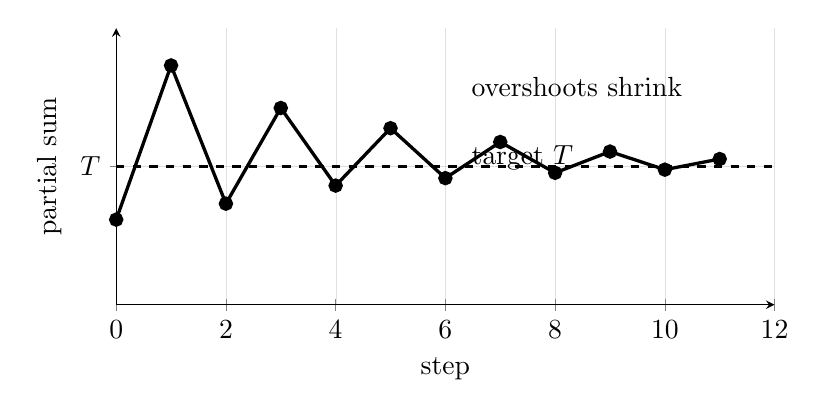
\begin{tikzpicture}
\begin{axis}[
    width=0.82\textwidth,
    height=0.42\textwidth,
    xmin=0, xmax=12,
    ymin=-0.8, ymax=1.8,
    axis lines=left,
    xlabel={step},
    ylabel={partial sum},
    xtick={0,2,4,6,8,10,12},
    ytick={0.5},
    yticklabels={\(T\)},
    grid=both,
    grid style={line width=.1pt, draw=gray!25},
]
\addplot[thick, dashed, domain=0:12, samples=2] {0.5};
\addplot[very thick, mark=*] coordinates {
    (0,0)
    (1,1.45)
    (2,0.15)
    (3,1.05)
    (4,0.32)
    (5,0.86)
    (6,0.39)
    (7,0.73)
    (8,0.44)
    (9,0.64)
    (10,0.47)
    (11,0.57)
};
\node[anchor=west] at (axis cs:6.3,1.25) {overshoots shrink};
\node[anchor=west] at (axis cs:6.3,0.58) {target \(T\)};
\end{axis}
\end{tikzpicture}
\caption{The Riemann rearrangement idea: alternate above and below a target, with shrinking overshoots.}
\label{fig:riemann-rearrangement-idea}
\end{figure}

This theorem is one of the clearest signs that infinity changes the rules.  A finite sum
cannot be rearranged to become a different number.  A conditionally convergent infinite
sum can.

\subsection{Why absolute convergence is safer}
\label{subsec:why-absolute-convergence-safer}

Absolute convergence prevents this danger.

\begin{quote}
\textbf{Rearrangements of absolutely convergent series.}
If

\[
\sum_{k=1}^{\infty}a_k
\]

converges absolutely, then every rearrangement of the series converges to the same sum.
\end{quote}

\paragraph{Proof idea.}
Let

\[
S=\sum_{k=1}^{\infty}a_k
\]

and suppose

\[
\sum_{k=1}^{\infty}|a_k|
\]

converges.

Given an error tolerance \(\varepsilon>0\), choose \(N\) so large that the absolute tail is
small:

\[
\sum_{k=N+1}^{\infty}|a_k|<\varepsilon.
\]

Now take any rearrangement of the series.  Go far enough in the rearranged partial sums
so that all of the first \(N\) original terms

\[
a_1,a_2,\ldots,a_N
\]

have appeared.

After that point, the only possible difference between the rearranged partial sum and
the full sum \(S\) comes from terms in the tail

\[
a_{N+1},a_{N+2},\ldots.
\]

The total absolute size of that tail is less than \(\varepsilon\).  Therefore the rearranged
partial sums must stay within \(\varepsilon\) of \(S\).

Since \(\varepsilon\) was arbitrary, the rearranged series converges to \(S\).

\[
\boxed{
\text{Absolute convergence makes the order irrelevant.}
}
\]

This is why absolute convergence is stronger than ordinary convergence.  It says the
series has finite total size, not merely a lucky cancellation pattern.

The next section collects the main traps in this chapter.  Each trap comes from using a
test after forgetting one of its hypotheses.

\section{Warning examples}
\label{sec:series-warning-examples}

Series tests are not recipes to apply by reflex.  Each test has hypotheses, and those
hypotheses are part of the mathematics.

This section collects the main warnings before we leave numerical series.

\[
\boxed{
\text{A series test used without its hypotheses is not a test.}
}
\]

\subsection{Terms tend to zero, but the series diverges}
\label{subsec:warning-terms-zero-series-diverges}

The most common mistake is to think that

\[
a_k\to0
\]

is enough to make

\[
\sum_{k=1}^{\infty}a_k
\]

converge.

It is not.

The harmonic series is the permanent counterexample:

\[
\sum_{k=1}^{\infty}\frac1k
=
1+\frac12+\frac13+\frac14+\cdots.
\]

The terms satisfy

\[
\frac1k\to0.
\]

But the series diverges.

Recall the doubled-block proof:

\[
1
+\frac12
+\left(\frac13+\frac14\right)
+\left(\frac15+\frac16+\frac17+\frac18\right)
+\cdots.
\]

Each doubled block contributes at least

\[
\frac12.
\]

So the partial sums grow beyond every bound.

\[
\boxed{
a_k\to0 \text{ is necessary for convergence, but not sufficient.}
}
\]

The term test is only a divergence test:

\[
\boxed{
a_k\not\to0
\quad\Longrightarrow\quad
\sum a_k \text{ diverges.}
}
\]

It has no converse.

\subsection{The Ratio Test can give no information}
\label{subsec:warning-ratio-test-no-information}

The Ratio Test says to compute

\[
L=
\lim_{k\to\infty}\left|\frac{a_{k+1}}{a_k}\right|.
\]

If

\[
L<1,
\]

we get absolute convergence.  If

\[
L>1,
\]

we get divergence.  If

\[
L=1,
\]

we get no information.

That last case is not a minor technicality.  It really means no information.

Compare two series.

First, the harmonic series:

\[
\sum_{k=1}^{\infty}\frac1k.
\]

Here

\[
a_k=\frac1k,
\]

so

\[
\left|\frac{a_{k+1}}{a_k}\right|
=
\frac{1}{k+1}\cdot k
=
\frac{k}{k+1}
\to1.
\]

The Ratio Test gives

\[
L=1.
\]

The series diverges, but the Ratio Test does not tell us that.

Now consider

\[
\sum_{k=1}^{\infty}\frac1{k^2}.
\]

Here

\[
a_k=\frac1{k^2},
\]

so

\[
\left|\frac{a_{k+1}}{a_k}\right|
=
\frac{1}{(k+1)^2}\cdot k^2
=
\left(\frac{k}{k+1}\right)^2
\to1.
\]

Again the Ratio Test gives

\[
L=1.
\]

This series converges.

So the same ratio-test result,

\[
L=1,
\]

occurs for one divergent series and one convergent series.

\[
\boxed{
\text{When the Ratio Test gives \(L=1\), switch tests.}
}
\]

For rational expressions in \(k\), comparison with a \(p\)-series is usually a better
choice than the Ratio Test.

\subsection{The Integral Test requires its hypotheses}
\label{subsec:warning-integral-test-hypotheses}

The Integral Test requires a function \(f\) that is

\[
\text{continuous, positive, and decreasing}
\]

on a tail interval such as \([1,\infty)\), with

\[
a_k=f(k).
\]

The proof compares positive rectangle areas with positive curved areas.  If the function
is not positive and decreasing, the geometric comparison may collapse.

Here is a sharp warning.

Let

\[
f(x)=-\sin^2(\pi x).
\]

This function is continuous and nonpositive.  At every positive integer \(k\),

\[
f(k)=-\sin^2(\pi k)=0.
\]

So the series formed by sampling \(f\) at the positive integers is

\[
\sum_{k=1}^{\infty}f(k)
=
0+0+0+\cdots,
\]

which converges to \(0\).

But the improper integral diverges to \(-\infty\):

\[
\int_1^b -\sin^2(\pi x)\,dx
=
-\int_1^b \sin^2(\pi x)\,dx.
\]

Using

\[
\sin^2(\pi x)=\frac{1-\cos(2\pi x)}{2},
\]

we get

\[
\int_1^b -\sin^2(\pi x)\,dx
=
-\frac{b-1}{2}
+
\frac{\sin(2\pi b)}{4\pi}.
\]

As

\[
b\to\infty,
\]

the term

\[
-\frac{b-1}{2}
\]

goes to \(-\infty\), while

\[
\frac{\sin(2\pi b)}{4\pi}
\]

stays bounded.  Therefore

\[
\int_1^\infty -\sin^2(\pi x)\,dx
\]

diverges.

So we have

\[
\sum_{k=1}^{\infty}f(k) \text{ converges}
\]

but

\[
\int_1^\infty f(x)\,dx \text{ diverges}.
\]

\[
\boxed{
\text{Sampling a function at integers and integrating it over an interval are not automatically equivalent.}
}
\]

The Integral Test works only because positivity and monotonicity let rectangles control
area.

\subsection{The Alternating Series Test requires decreasing term sizes}
\label{subsec:warning-alternating-test-decreasing}

The Alternating Series Test says that

\[
\sum_{k=1}^{\infty}(-1)^{k-1}b_k
\]

converges if

\[
b_k\ge0,
\qquad
b_{k+1}\le b_k,
\qquad
b_k\to0.
\]

The condition

\[
b_k\to0
\]

alone is not enough.  The decreasing condition organizes the cancellation.

Here is a counterexample.

Define

\[
b_{2m-1}=\frac1m,
\qquad
b_{2m}=\frac1{m^2},
\qquad
m=1,2,3,\ldots.
\]

Then

\[
b_k\to0.
\]

But the sequence \(\{b_k\}\) is not decreasing.  For instance,

\[
b_4=\frac14,
\qquad
b_5=\frac13,
\]

so

\[
b_5>b_4.
\]

Now form the alternating series

\[
\sum_{k=1}^{\infty}(-1)^{k-1}b_k.
\]

Group the terms in pairs:

\[
(b_1-b_2)+(b_3-b_4)+(b_5-b_6)+\cdots.
\]

Using the definition of \(b_k\), this becomes

\[
\left(1-1\right)
+
\left(\frac12-\frac14\right)
+
\left(\frac13-\frac19\right)
+
\left(\frac14-\frac1{16}\right)
+\cdots.
\]

The \(m\)-th pair is

\[
\frac1m-\frac1{m^2}.
\]

For \(m\ge2\),

\[
\frac1m-\frac1{m^2}
=
\frac{m-1}{m^2}
\ge
\frac1{2m}.
\]

Therefore the paired partial sums dominate

\[
\sum_{m=2}^{\infty}\frac1{2m},
\]

which diverges.

So the original alternating series diverges, even though

\[
b_k\to0.
\]

\[
\boxed{
\text{Alternating signs plus terms tending to zero are not enough.}
}
\]

The term sizes must decrease, at least eventually, for the Alternating Series Test to
apply.

\subsection{The final checklist}
\label{subsec:series-final-checklist}

Before deciding that a series converges or diverges, check the exact reason.

\begin{center}
\begin{tabular}{c|c}
\textbf{claim} & \textbf{what must be true} \\ \hline
\(\sum a_k\) converges by the term test & never; the term test proves only divergence \\[3pt]
\(\sum a_k\) diverges by the term test & \(a_k\not\to0\) \\[3pt]
\(\sum a_k\) converges by comparison & terms are eventually nonnegative and bounded by a convergent series \\[3pt]
\(\sum a_k\) diverges by comparison & terms are eventually at least a divergent positive series \\[3pt]
Integral Test applies & \(f\) is continuous, positive, decreasing, and \(a_k=f(k)\) \\[3pt]
Alternating Series Test applies & term sizes are nonnegative, decreasing, and tend to \(0\) \\[3pt]
Ratio or Root Test decides & the limit is less than \(1\) or greater than \(1\) \\[3pt]
absolute convergence holds & \(\sum |a_k|\) converges
\end{tabular}
\end{center}

The point is not to memorize a list of traps.  The point is to keep the meaning visible.

A series is an accumulated limit:

\[
\sum_{k=1}^{\infty}a_k
=
\lim_{n\to\infty}
(a_1+a_2+\cdots+a_n).
\]

Every test is a way to control that limit.

In the next chapter, the terms of the series will contain a variable:

\[
a_0+a_1x+a_2x^2+a_3x^3+\cdots.
\]

Then an infinite sum becomes a function.  That is where series stop being only numbers
and become a new way to represent \(e^x\), \(\sin x\), \(\cos x\), and many functions
whose antiderivatives cannot be written in elementary form.

\section{Chapter review and discovery problems}
\label{sec:chapter-review-series-discovery-problems}

This chapter began with a list:

\[
a_1,\ a_2,\ a_3,\ldots.
\]

Then we added the list:

\[
a_1+a_2+a_3+\cdots.
\]

That small change created a large question.  A sequence asks whether the terms settle
down.  A series asks whether the accumulated partial sums settle down.

\[
\boxed{
\sum_{k=1}^{\infty}a_k
=
\lim_{n\to\infty}
\sum_{k=1}^{n}a_k.
}
\]

Everything in this chapter is a way to understand that limit.

\subsection{The chapter in one picture}
\label{subsec:chapter-in-one-picture}

The main objects and questions are these.

\begin{center}
\begin{tabular}{c|c|c}
\textbf{object} & \textbf{what it means} & \textbf{main question} \\ \hline
sequence \(\{a_n\}\) & an infinite list & does \(a_n\) approach a limit? \\[3pt]
series \(\sum a_k\) & a limit of partial sums & do the partial sums approach a limit? \\[3pt]
positive series & no cancellation & are the partial sums bounded above? \\[3pt]
alternating series & organized cancellation & do decreasing term sizes force convergence? \\[3pt]
absolute series \(\sum |a_k|\) & total size & does the series converge without cancellation?
\end{tabular}
\end{center}

The most important warning is still the harmonic series:

\[
\sum_{k=1}^{\infty}\frac1k
\]

diverges, even though

\[
\frac1k\to0.
\]

So the term test has only one safe direction:

\[
\boxed{
a_k\not\to0
\quad\Longrightarrow\quad
\sum a_k \text{ diverges.}
}
\]

If

\[
a_k\to0,
\]

we must keep working.

\subsection{Skills: choosing series tests}
\label{subsec:skills-choosing-series-tests}

A series often tells us which test it wants.  The first step is to look at the shape of the
term.

\begin{center}
\begin{tabular}{c|l}
\textbf{what you see} & \textbf{what to try} \\ \hline
terms do not approach \(0\) & term test for divergence \\[3pt]
\(ar^k\) or constant ratio & geometric series \\[3pt]
visible cancellation & telescoping \\[3pt]
positive terms involving powers of \(k\) & \(p\)-series, comparison, integral test \\[3pt]
rational expression in \(k\) & limit comparison with leading powers \\[3pt]
\((-1)^k\) with decreasing term sizes & Alternating Series Test \\[3pt]
factorials or exponentials & Ratio Test \\[3pt]
a \(k\)-th power & Root Test
\end{tabular}
\end{center}

This table is a guide, not a law.  If one test gives no information, use another.

\paragraph{Review example: leading powers.}
Decide whether

\[
\sum_{k=1}^{\infty}\frac{4k^2+1}{k^4+3}
\]

converges.

For large \(k\),

\[
\frac{4k^2+1}{k^4+3}
\]

behaves like

\[
\frac{4k^2}{k^4}=\frac4{k^2}.
\]

Compare with

\[
b_k=\frac1{k^2}.
\]

Let

\[
a_k=\frac{4k^2+1}{k^4+3}.
\]

Then

\[
\frac{a_k}{b_k}
=
\frac{4k^2+1}{k^4+3}\cdot k^2
=
\frac{4k^4+k^2}{k^4+3}.
\]

Divide numerator and denominator by \(k^4\):

\[
\frac{4+\frac1{k^2}}{1+\frac3{k^4}}\to4.
\]

Since

\[
0<4<\infty
\]

and

\[
\sum_{k=1}^{\infty}\frac1{k^2}
\]

converges, the given series converges.

\[
\boxed{
\sum_{k=1}^{\infty}\frac{4k^2+1}{k^4+3}
\text{ converges.}
}
\]

\paragraph{Review example: conditional convergence.}
Decide whether

\[
\sum_{k=1}^{\infty}(-1)^{k-1}\frac{k}{k^2+1}
\]

converges absolutely, conditionally, or not at all.

First test absolute convergence:

\[
\sum_{k=1}^{\infty}
\left|(-1)^{k-1}\frac{k}{k^2+1}\right|
=
\sum_{k=1}^{\infty}\frac{k}{k^2+1}.
\]

For large \(k\),

\[
\frac{k}{k^2+1}
\]

behaves like

\[
\frac1k.
\]

Use limit comparison with \(1/k\):

\[
\frac{\frac{k}{k^2+1}}{\frac1k}
=
\frac{k^2}{k^2+1}
\to1.
\]

Since the harmonic series diverges, the absolute-value series diverges.

Now test the original alternating series.  Let

\[
b_k=\frac{k}{k^2+1}.
\]

Then

\[
b_k\to0.
\]

Also, \(b_k\) is decreasing for \(k\ge1\).  One way to see this is to compare consecutive
terms:

\[
\frac{k+1}{(k+1)^2+1}
\le
\frac{k}{k^2+1}
\]

is equivalent, after multiplying by positive denominators, to

\[
(k+1)(k^2+1)\le k((k+1)^2+1).
\]

Expanding gives

\[
k^3+k^2+k+1\le k^3+2k^2+2k,
\]

which reduces to

\[
1\le k^2+k.
\]

This is true for \(k\ge1\).

So the Alternating Series Test applies.  The original series converges, but not
absolutely.

\[
\boxed{
\sum_{k=1}^{\infty}(-1)^{k-1}\frac{k}{k^2+1}
\text{ converges conditionally.}
}
\]

\paragraph{Review example: factorials.}
Decide whether

\[
\sum_{k=1}^{\infty}\frac{k!}{100^k}
\]

converges.

Use the Ratio Test:

\[
a_k=\frac{k!}{100^k}.
\]

Then

\[
\frac{a_{k+1}}{a_k}
=
\frac{(k+1)!}{100^{k+1}}\cdot\frac{100^k}{k!}
=
\frac{k+1}{100}.
\]

As \(k\to\infty\),

\[
\frac{k+1}{100}\to\infty.
\]

The Ratio Test gives divergence.

\[
\boxed{
\sum_{k=1}^{\infty}\frac{k!}{100^k}
\text{ diverges.}
}
\]

The factorial eventually grows faster than the exponential \(100^k\).

\paragraph{Review example: a \(k\)-th power.}
Decide whether

\[
\sum_{k=1}^{\infty}
\left(\frac{2k+1}{3k+5}\right)^k
\]

converges.

Use the Root Test.  Let

\[
a_k=
\left(\frac{2k+1}{3k+5}\right)^k.
\]

Then

\[
\sqrt[k]{|a_k|}
=
\frac{2k+1}{3k+5}
=
\frac{2+\frac1k}{3+\frac5k}.
\]

Therefore

\[
\lim_{k\to\infty}\sqrt[k]{|a_k|}
=
\frac23.
\]

Since

\[
\frac23<1,
\]

the series converges absolutely.

\[
\boxed{
\sum_{k=1}^{\infty}
\left(\frac{2k+1}{3k+5}\right)^k
\text{ converges.}
}
\]

\subsection{Concept check}
\label{subsec:series-concept-check}

Answer these without doing long computations.

\begin{enumerate}
\item What is the difference between the sequence \(\{a_n\}\) and the series
\[
\sum_{n=1}^{\infty}a_n?
\]

\item If
\[
\sum_{n=1}^{\infty}a_n
\]
converges, what must be true about \(a_n\)?

\item Give an example showing that
\[
a_n\to0
\]
does not guarantee that
\[
\sum a_n
\]
converges.

\item Why are the partial sums of a positive series increasing?

\item What does it mean for a series to converge absolutely?

\item What does it mean for a series to converge conditionally?

\item Why does the Ratio Test give no conclusion when the ratio limit is \(1\)?

\item What hypotheses must be checked before using the Integral Test?

\item What hypotheses must be checked before using the Alternating Series Test?

\item Why can a conditionally convergent series change sum when rearranged, while an
absolutely convergent series cannot?
\end{enumerate}

\subsection{Skills practice}
\label{subsec:series-skills-practice}

For each sequence, determine whether it converges.  If it converges, find the limit.

\begin{enumerate}
\item
\[
a_n=\frac{3n+1}{5n-2}
\]

\item
\[
a_n=(-1)^n\frac{n}{n+1}
\]

\item
\[
a_n=\frac{\ln n}{n}
\]

\item
\[
a_0=1,
\qquad
a_{n+1}=\frac{a_n+5}{2}.
\]

\item
\[
a_0=1,
\qquad
a_{n+1}=2-a_n.
\]
\end{enumerate}

For each series, decide whether it converges or diverges.  If it converges, decide
whether the convergence is absolute or conditional when signs are involved.

\begin{enumerate}
\setcounter{enumi}{5}

\item
\[
\sum_{k=1}^{\infty}\frac{5}{3^k}
\]

\item
\[
\sum_{k=1}^{\infty}\frac{k^2+1}{k^4+1}
\]

\item
\[
\sum_{k=1}^{\infty}\frac{2k+1}{k+4}
\]

\item
\[
\sum_{k=1}^{\infty}(-1)^{k-1}\frac1{k^{2/3}}
\]

\item
\[
\sum_{k=1}^{\infty}(-1)^k\frac1{k^2}
\]

\item
\[
\sum_{k=1}^{\infty}\frac{k^3}{5^k}
\]

\item
\[
\sum_{k=1}^{\infty}\frac{k!}{k^k}
\]

\item
\[
\sum_{k=1}^{\infty}
\left(\frac{k+1}{2k+3}\right)^k
\]

\item
\[
\sum_{k=2}^{\infty}\frac1{k\ln k}
\]

\item
\[
\sum_{k=1}^{\infty}\frac{\sin^2 k}{k^2}
\]

\item
\[
\sum_{k=1}^{\infty}(-1)^{k-1}\frac{k+1}{k^2+1}
\]

\item
\[
\sum_{k=1}^{\infty}\left(\sqrt{k+1}-\sqrt{k}\right)
\]

\item
\[
\sum_{k=1}^{\infty}\frac1{k(k+3)}
\]

\item
\[
\sum_{k=1}^{\infty}\frac{2^k+k}{3^k}
\]

\item
\[
\sum_{k=1}^{\infty}\frac{10^k}{k!}
\]
\end{enumerate}

\subsection{Project: estimate sums with rigorous error bounds}
\label{subsec:project-estimate-sums-rigorous-error-bounds}

Numerical answers are useful only when we know how much to trust them.  In this
project, every approximation must come with an error bound.

Choose at least two of the following sums.

\[
A=\sum_{k=1}^{\infty}\frac1{k^2},
\]

\[
B=\sum_{k=1}^{\infty}(-1)^{k-1}\frac1{k^2},
\]

\[
C=\sum_{k=0}^{\infty}3\left(\frac14\right)^k,
\]

\[
D=\sum_{k=1}^{\infty}\frac{k^2}{3^k}.
\]

For each chosen sum:

\begin{enumerate}
\item Explain which convergence test applies.

\item Compute a partial sum \(S_N\).

\item Give an interval
\[
\text{lower bound}\le S\le \text{upper bound}
\]
that is guaranteed to contain the true sum.

\item Choose \(N\) large enough so that the length of your interval is less than
\[
0.001.
\]

\item State your approximation in the form
\[
S\approx S_N
\]
with a rigorous error statement.
\end{enumerate}

For the geometric sum \(C\), use the exact tail formula.  For \(A\), use the integral-test
remainder estimate.  For \(B\), use the alternating-series error estimate.  For \(D\), use
the Ratio Test to find a geometric bound for the tail after some point.

\paragraph{A sample format.}
For

\[
S=\sum_{k=1}^{\infty}\frac1{k^2},
\]

the integral-test remainder estimate gives

\[
\int_{N+1}^{\infty}\frac1{x^2}\,dx
\le
S-S_N
\le
\int_N^{\infty}\frac1{x^2}\,dx.
\]

So

\[
\frac1{N+1}
\le
S-S_N
\le
\frac1N.
\]

Thus

\[
S_N+\frac1{N+1}
\le
S
\le
S_N+\frac1N.
\]

This is an honest interval for the true sum.

\subsection{Computing: numerical partial sums can mislead}
\label{subsec:computing-partial-sums-can-mislead}

A computer can add many terms quickly.  That is helpful, but it can also create false
confidence.

Compare the two series

\[
\sum_{k=1}^{\infty}\frac1{k^{0.99}}
\qquad\text{and}\qquad
\sum_{k=1}^{\infty}\frac1{k^{1.01}}.
\]

They look almost the same for a long time.  Their partial sums grow slowly.

\begin{center}
\begin{tabular}{c|c|c}
\textbf{\(N\)} &
\(\displaystyle \sum_{k=1}^{N}\frac1{k^{0.99}}\) &
\(\displaystyle \sum_{k=1}^{N}\frac1{k^{1.01}}\) \\ \hline
\(10\) & \(2.9561\) & \(2.9023\) \\
\(100\) & \(5.2946\) & \(5.0835\) \\
\(1000\) & \(7.7290\) & \(7.2530\) \\
\(10000\) & \(10.2244\) & \(9.3769\)
\end{tabular}
\end{center}

The numbers are close.  A graph of the first several thousand partial sums might make
both series look as if they are slowly leveling off.

But the \(p\)-series test says something decisive:

\[
\sum_{k=1}^{\infty}\frac1{k^{0.99}}
\]

diverges because

\[
0.99<1,
\]

while

\[
\sum_{k=1}^{\infty}\frac1{k^{1.01}}
\]

converges because

\[
1.01>1.
\]

The difference between the exponents is only \(0.02\), but it changes the infinite
behavior completely.

\begin{quote}
\textbf{Computing lesson.}
A long list of partial sums can suggest a pattern, but it cannot replace a theorem.
Slow divergence can look like convergence for a very long time.
\end{quote}

\paragraph{Computing task.}
Use a spreadsheet or computer program to compute partial sums for

\[
\sum_{k=1}^{N}\frac1{k},
\qquad
\sum_{k=1}^{N}\frac1{k^{1.01}},
\qquad
\sum_{k=1}^{N}\frac1{k^2}
\]

for

\[
N=10,\ 100,\ 1000,\ 10000.
\]

Then answer:

\begin{enumerate}
\item Which sums appear to grow quickly?

\item Which sums appear to grow slowly?

\item Which series actually converge?

\item For the convergent series, use an error estimate to say how far the partial sum
\(S_{10000}\) might still be from the true sum.

\item Explain why numerical evidence alone is not enough to decide convergence.
\end{enumerate}

\subsection{Discovery problems}
\label{subsec:series-discovery-problems}

These problems ask you to experiment before proving.

\begin{enumerate}
\item \textbf{A family near the harmonic boundary.}
For several values of \(p\) near \(1\), compute partial sums of
\[
\sum_{k=1}^{N}\frac1{k^p}.
\]
Try
\[
p=0.9,\quad p=0.99,\quad p=1,\quad p=1.01,\quad p=1.1.
\]
Which values produce convergent series?  Which produce divergent series?  How easy is
it to guess correctly from partial sums alone?

\item \textbf{Alternating error.}
For
\[
S=\sum_{k=1}^{\infty}(-1)^{k-1}\frac1k,
\]
compute \(S_n\) for
\[
n=10,\ 100,\ 1000.
\]
Use the alternating error estimate to give a guaranteed interval for \(S\).  How many
terms are needed for an error less than \(10^{-4}\)?

\item \textbf{A telescoping experiment.}
Find constants \(A\) and \(B\) such that
\[
\frac1{k(k+3)}
=
\frac{A}{k}+\frac{B}{k+3}.
\]
Use this to evaluate
\[
\sum_{k=1}^{\infty}\frac1{k(k+3)}.
\]
Be careful: the cancellation leaves several initial and final terms.

\item \textbf{A ratio-test family.}
For each positive number \(c\), consider
\[
\sum_{k=1}^{\infty}\frac{k^2}{c^k}.
\]
Use the Ratio Test to decide for which values of \(c\) the series converges.

\item \textbf{Rearranging a conditionally convergent series.}
Take the alternating harmonic series.  Write the terms in the pattern
\[
\text{three positive terms, then one negative term}.
\]
Compute several grouped partial sums.  Do they appear to approach the original sum?
What does this suggest about conditional convergence?
\end{enumerate}

\subsection{Hook: some infinite sums are functions}
\label{subsec:hook-infinite-sums-as-functions}

This chapter studied numerical series:

\[
\sum_{k=1}^{\infty}a_k.
\]

The next chapter lets the terms depend on \(x\):

\[
a_0+a_1x+a_2x^2+a_3x^3+\cdots.
\]

Then the infinite sum is no longer just a number.  It is a function.

This changes the story.  We will ask:

\[
\text{For which \(x\)-values does the series converge?}
\]

and then:

\[
\text{Can we differentiate or integrate the series term by term?}
\]

That question leads to power series, Taylor polynomials, and the promised bridge to

\[
e^x,
\qquad
\sin x,
\qquad
\cos x,
\qquad
e^{i\theta}.
\]

The next chapter begins with the simplest infinite polynomial:

\[
1+x+x^2+x^3+\cdots.
\]